%&preformat-synopsis
\RequirePackage[l2tabu,orthodox]{nag} % Раскомментировав, можно в логе получать рекомендации относительно правильного использования пакетов и предупреждения об устаревших и нерекомендуемых пакетах
\PassOptionsToPackage{bookmarks=false}{hyperref}
\documentclass[a5paper,10pt,twoside,openany,article]{memoir} %,draft
%%%% Основные сведения %%%
\newcommand{\thesisAuthor}             % Диссертация, ФИО автора
{%
    \texorpdfstring{% \texorpdfstring takes two arguments and uses the first for (La)TeX and the second for pdf
        Филатов Сергей Васильевич% так будет отображаться на титульном листе или в тексте, где будет использоваться переменная
    }{%
        Филатов, Сергей Васильевич% эта запись для свойств pdf-файла. В таком виде, если pdf будет обработан программами для сбора библиографических сведений, будет правильно представлена фамилия.
    }%
}
\newcommand{\thesisAuthorShort}        % Диссертация, ФИО автора инициалами
{С.В.~Филатов}

\newcommand{\thesisUdk}                % Диссертация, УДК
{532.59}
\newcommand{\thesisTitle}              % Диссертация, название
{\texorpdfstring{\MakeUppercase{Волны и вихри на свободной поверхности жидкости}}{Название диссертационной работы}}
\newcommand{\thesisSpecialtyNumber}    % Диссертация, специальность, номер
{\texorpdfstring{01.04.07}}
\newcommand{\thesisSpecialtyTitle}     % Диссертация, специальность, название
{физика конденсированного состояния}
\newcommand{\thesisDegree}             % Диссертация, ученая степень
{кандидата физико-математических наук}
\newcommand{\thesisDegreeShort}        % Диссертация, ученая степень, краткая запись
{канд. физ.-мат. наук}
\newcommand{\thesisCity}               % Диссертация, город написания диссертации
{Черноголовка}
\newcommand{\thesisYear}               % Диссертация, год написания диссертации
{2017}
\newcommand{\thesisOrganization}       % Диссертация, организация
{Федеральное государственное бюджетное учреждение науки Институт физики твердого тела Российской академии наук}
\newcommand{\thesisOrganizationShort}  % Диссертация, краткое название организации для доклада
{ИФТТ РАН}

\newcommand{\thesisInOrganization}     % Диссертация, организация в предложном падеже: Работа выполнена в ...
{\todo{учреждении, в~котором выполнялась данная диссертационная работа}}

\newcommand{\supervisorFio}            % Научный руководитель, ФИО
{Левченко Александр Алексеевич}
\newcommand{\supervisorRegalia}        % Научный руководитель, регалии
{доктор физико-математических наук}
\newcommand{\supervisorFioShort}       % Научный руководитель, ФИО
{{А.А.~Левченко}}
\newcommand{\supervisorRegaliaShort}   % Научный руководитель, регалии
{докт. физ.-мат. наук}


\newcommand{\opponentOneFio}           % Оппонент 1, ФИО
{\todo{Фамилия Имя Отчество}}
\newcommand{\opponentOneRegalia}       % Оппонент 1, регалии
{\todo{доктор физико-математических наук, профессор}}
\newcommand{\opponentOneJobPlace}      % Оппонент 1, место работы
{\todo{Не очень длинное название для места работы}}
\newcommand{\opponentOneJobPost}       % Оппонент 1, должность
{\todo{старший научный сотрудник}}

\newcommand{\opponentTwoFio}           % Оппонент 2, ФИО
{\todo{Фамилия Имя Отчество}}
\newcommand{\opponentTwoRegalia}       % Оппонент 2, регалии
{\todo{кандидат физико-математических наук}}
\newcommand{\opponentTwoJobPlace}      % Оппонент 2, место работы
{\todo{Основное место работы c длинным длинным длинным длинным названием}}
\newcommand{\opponentTwoJobPost}       % Оппонент 2, должность
{\todo{старший научный сотрудник}}

\newcommand{\leadingOrganizationTitle} % Ведущая организация, дополнительные строки
{\todo{Федеральное государственное бюджетное образовательное учреждение высшего профессионального образования с~длинным длинным длинным длинным названием}}

\newcommand{\defenseDate}              % Защита, дата
{\todo{DD mmmmmmmm YYYY~г.~в~XX часов}}
\newcommand{\defenseCouncilNumber}     % Защита, номер диссертационного совета
{\todo{Д\,123.456.78}}
\newcommand{\defenseCouncilTitle}      % Защита, учреждение диссертационного совета
{\todo{Название учреждения}}
\newcommand{\defenseCouncilAddress}    % Защита, адрес учреждение диссертационного совета
{\todo{Адрес}}
\newcommand{\defenseCouncilPhone}      % Телефон для справок
{\todo{+7~(0000)~00-00-00}}

\newcommand{\defenseSecretaryFio}      % Секретарь диссертационного совета, ФИО
{\todo{Фамилия Имя Отчество}}
\newcommand{\defenseSecretaryRegalia}  % Секретарь диссертационного совета, регалии
{\todo{д-р~физ.-мат. наук}}            % Для сокращений есть ГОСТы, например: ГОСТ Р 7.0.12-2011 + http://base.garant.ru/179724/#block_30000

\newcommand{\synopsisLibrary}          % Автореферат, название библиотеки
{\todo{Название библиотеки}}
\newcommand{\synopsisDate}             % Автореферат, дата рассылки
{\todo{DD mmmmmmmm YYYY года}}

% To avoid conflict with beamer class use \providecommand
\providecommand{\keywords}%            % Ключевые слова для метаданных PDF диссертации и автореферата
{}      % Основные сведения

%% Режим черновика
\makeatletter
\@ifundefined{c@draft}{
  \newcounter{draft}
  \setcounter{draft}{0}  % 0 --- чистовик (максимальное соблюдение ГОСТ)
                         % 1 --- черновик (отклонения от ГОСТ, но быстрая сборка итоговых PDF)
}{}
\makeatother

%% Библиография

%% Внимание! При использовании bibtex8 необходимо удалить все
%% цитирования из  ../common/characteristic.tex
%\newcounter{bibliosel}
%\setcounter{bibliosel}{1}           % 0 --- встроенная реализация с загрузкой файла через движок bibtex8; 1 --- реализация пакетом biblatex через движок biber
          % общие настройки шаблона
%%% Проверка используемого TeX-движка %%%
\usepackage{iftex}[2013/04/04]
\newif\ifxetexorluatex   % определяем новый условный оператор (http://tex.stackexchange.com/a/47579/79756)
\ifXeTeX
    \xetexorluatextrue
\else
    \ifLuaTeX
        \xetexorluatextrue
    \else
        \xetexorluatexfalse
    \fi
\fi

\RequirePackage{etoolbox}[2015/08/02]               % Для продвинутой проверки разных условий

%%% Поля и разметка страницы %%%
\usepackage{pdflscape}                              % Для включения альбомных страниц
\usepackage[left=2cm,right=2cm]{geometry}                               % Для последующего задания полей

%%% Математические пакеты %%%
\usepackage{amsthm,amsfonts,amsmath,amssymb,amscd}  % Математические дополнения от AMS
\usepackage{mathtools}                              % Добавляет окружение multlined

%%%% Установки для размера шрифта 14 pt %%%%
%% Формирование переменных и констант для сравнения (один раз для всех подключаемых файлов)%%
%% должно располагаться до вызова пакета fontspec или polyglossia, потому что они сбивают его работу
\newlength{\curtextsize}
\newlength{\bigtextsize}
\setlength{\bigtextsize}{13.9pt}

\makeatletter
%\show\f@size                                       % неплохо для отслеживания, но вызывает стопорение процесса, если документ компилируется без команды  -interaction=nonstopmode 
\setlength{\curtextsize}{\f@size pt}
\makeatother

%%% Кодировки и шрифты %%%
\ifxetexorluatex
    \usepackage{polyglossia}[2014/05/21]            % Поддержка многоязычности (fontspec подгружается автоматически)
\else
    \RequirePDFTeX                                  % tests for PDFTEX use and throws an error if a different engine is being used
   %%% Решение проблемы копирования текста в буфер кракозябрами
%    \input glyphtounicode.tex
%    \input glyphtounicode-cmr.tex %from pdfx package
%    \pdfgentounicode=1
    \usepackage{cmap}                               % Улучшенный поиск русских слов в полученном pdf-файле
    \defaulthyphenchar=127                          % Если стоит до fontenc, то переносы не впишутся в выделяемый текст при копировании его в буфер обмена
    \usepackage[T2A]{fontenc}                       % Поддержка русских букв
    \usepackage[utf8]{inputenc}[2014/04/30]         % Кодировка utf8
    \usepackage[english, russian]{babel}[2014/03/24]% Языки: русский, английский
    \IfFileExists{pscyr.sty}{\usepackage{pscyr}}{}  % Красивые русские шрифты
\fi

%%% Оформление абзацев %%%
\usepackage{indentfirst}                            % Красная строка

%%% Цвета %%%
\usepackage[dvipsnames,usenames]{color}
\usepackage{colortbl}
%\usepackage[dvipsnames, table, hyperref, cmyk]{xcolor} % Вероятно, более новый вариант, вместо предыдущих двух строк. Конвертация всех цветов в cmyk заложена как удовлетворение возможного требования типографий. Возможно конвертирование и в rgb.

%%% Таблицы %%%
\usepackage{longtable}                              % Длинные таблицы
\usepackage{multirow,makecell}                      % Улучшенное форматирование таблиц

%%% Общее форматирование
\usepackage{soulutf8}                               % Поддержка переносоустойчивых подчёркиваний и зачёркиваний
\usepackage{icomma}                                 % Запятая в десятичных дробях


%%% Гиперссылки %%%
\usepackage{hyperref}[2012/11/06]

%%% Изображения %%%
\usepackage{graphicx}[2014/04/25]                   % Подключаем пакет работы с графикой

%%% Списки %%%
\usepackage{enumitem}

%%% Подписи %%%
\usepackage{caption}[2013/05/02]                    % Для управления подписями (рисунков и таблиц) % Может управлять номерами рисунков и таблиц с caption %Иногда может управлять заголовками в списках рисунков и таблиц
\usepackage{subcaption}[2013/02/03]                 % Работа с подрисунками и подобным

%%% Счётчики %%%
\usepackage[figure,table]{totalcount}               % Счётчик рисунков и таблиц
\usepackage{totcount}                               % Пакет создания счётчиков на основе последнего номера подсчитываемого элемента (может требовать дважды компилировать документ)
\usepackage{totpages}                               % Счётчик страниц, совместимый с hyperref (ссылается на номер последней страницы). Желательно ставить последним пакетом в преамбуле

%%% Продвинутое управление групповыми ссылками (пока только формулами) %%%
\ifxetexorluatex
    \usepackage{cleveref}                           % cleveref корректно считывает язык из настроек polyglossia
\else
    \usepackage[russian]{cleveref}                  % cleveref имеет сложности со считыванием языка из babel. Такое решение русификации вывода выбрано вместо определения в documentclass из опасности что-то лишнее передать во все остальные пакеты, включая библиографию.
\fi
\creflabelformat{equation}{#2#1#3}                  % Формат по умолчанию ставил круглые скобки вокруг каждого номера ссылки, теперь просто номера ссылок без какого-либо дополнительного оформления


\ifnumequal{\value{draft}}{1}{% Черновик
    \usepackage[firstpage]{draftwatermark}
    \SetWatermarkText{DRAFT}
    \SetWatermarkFontSize{14pt}
    \SetWatermarkScale{15}
    \SetWatermarkAngle{45}
}{}

       % Пакеты общие для диссертации и автореферата
\input{Synopsis/synpackages}  % Пакеты для автореферата
\usepackage{tabu, tabulary}  %таблицы с автоматически подбирающейся шириной столбцов
\usepackage{fr-longtable}    %ради \endlasthead
% Листинги с исходным кодом программ
\usepackage{fancyvrb}
\usepackage{listings}
\lccode`\~=0\relax %Без этого хака из-за особенностей пакета listings перестают работать конструкции с \MakeLowercase и т. п. в (xe|lua)latex

% Русская традиция начертания греческих букв
\usepackage{upgreek} % прямые греческие ради русской традиции

% Микротипографика
%\ifnumequal{\value{draft}}{0}{% Только если у нас режим чистовика
%    \usepackage[final]{microtype}[2016/05/14] % улучшает представление букв и слов в строках, может помочь при наличии отдельно висящих слов
%}{}

% Отметка о версии черновика на каждой странице
% Чтобы работало надо в своей локальной копии по инструкции
% https://www.ctan.org/pkg/gitinfo2 создать небходимые файлы в папке
% ./git/hooks
% If you’re familiar with tweaking git, you can probably work it out for
% yourself. If not, I suggest you follow these steps:
% 1. First, you need a git repository and working tree. For this example,
% let’s suppose that the root of the working tree is in ~/compsci
% 2. Copy the file post-xxx-sample.txt (which is in the same folder of
% your TEX distribution as this pdf) into the git hooks directory in your
% working copy. In our example case, you should end up with a file called
% ~/compsci/.git/hooks/post-checkout
% 3. If you’re using a unix-like system, don’t forget to make the file executable.
% Just how you do this is outside the scope of this manual, but one
% possible way is with commands such as this:
% chmod g+x post-checkout.
% 4. Test your setup with “git checkout master” (or another suitable branch
% name). This should generate copies of gitHeadInfo.gin in the directories
% you intended.
% 5. Now make two more copies of this file in the same directory (hooks),
% calling them post-commit and post-merge, and you’re done. As before,
% users of unix-like systems should ensure these files are marked as
% executable.
\ifnumequal{\value{draft}}{1}{% Черновик
   \IfFileExists{.git/gitHeadInfo.gin}{                                        
      \usepackage[mark,pcount]{gitinfo2}
      \renewcommand{\gitMark}{rev.\gitAbbrevHash\quad\gitCommitterEmail\quad\gitAuthorIsoDate}
      \renewcommand{\gitMarkFormat}{\color{Gray}\small\bfseries}
   }{}
}{} % Пакеты для специфических пользовательских задач

\input{common/newnames}       % Новые переменные, которые могут использоваться во всём проекте
%% Режим черновика
\makeatletter
\@ifundefined{c@draft}{
  \newcounter{draft}
  \setcounter{draft}{0}  % 0 --- чистовик (максимальное соблюдение ГОСТ)
                         % 1 --- черновик (отклонения от ГОСТ, но быстрая сборка итоговых PDF)
}{}
\makeatother

%% Библиография

%% Внимание! При использовании bibtex8 необходимо удалить все
%% цитирования из  ../common/characteristic.tex
%\newcounter{bibliosel}
%\setcounter{bibliosel}{1}           % 0 --- встроенная реализация с загрузкой файла через движок bibtex8; 1 --- реализация пакетом biblatex через движок biber
        % Упрощённые настройки шаблона 

%%% Основные сведения %%%
\newcommand{\thesisAuthor}             % Диссертация, ФИО автора
{%
    \texorpdfstring{% \texorpdfstring takes two arguments and uses the first for (La)TeX and the second for pdf
        Филатов Сергей Васильевич% так будет отображаться на титульном листе или в тексте, где будет использоваться переменная
    }{%
        Филатов, Сергей Васильевич% эта запись для свойств pdf-файла. В таком виде, если pdf будет обработан программами для сбора библиографических сведений, будет правильно представлена фамилия.
    }%
}
\newcommand{\thesisAuthorShort}        % Диссертация, ФИО автора инициалами
{С.В.~Филатов}

\newcommand{\thesisUdk}                % Диссертация, УДК
{532.59}
\newcommand{\thesisTitle}              % Диссертация, название
{\texorpdfstring{\MakeUppercase{Волны и вихри на свободной поверхности жидкости}}{Название диссертационной работы}}
\newcommand{\thesisSpecialtyNumber}    % Диссертация, специальность, номер
{\texorpdfstring{01.04.07}}
\newcommand{\thesisSpecialtyTitle}     % Диссертация, специальность, название
{физика конденсированного состояния}
\newcommand{\thesisDegree}             % Диссертация, ученая степень
{кандидата физико-математических наук}
\newcommand{\thesisDegreeShort}        % Диссертация, ученая степень, краткая запись
{канд. физ.-мат. наук}
\newcommand{\thesisCity}               % Диссертация, город написания диссертации
{Черноголовка}
\newcommand{\thesisYear}               % Диссертация, год написания диссертации
{2017}
\newcommand{\thesisOrganization}       % Диссертация, организация
{Федеральное государственное бюджетное учреждение науки Институт физики твердого тела Российской академии наук}
\newcommand{\thesisOrganizationShort}  % Диссертация, краткое название организации для доклада
{ИФТТ РАН}

\newcommand{\thesisInOrganization}     % Диссертация, организация в предложном падеже: Работа выполнена в ...
{\todo{учреждении, в~котором выполнялась данная диссертационная работа}}

\newcommand{\supervisorFio}            % Научный руководитель, ФИО
{Левченко Александр Алексеевич}
\newcommand{\supervisorRegalia}        % Научный руководитель, регалии
{доктор физико-математических наук}
\newcommand{\supervisorFioShort}       % Научный руководитель, ФИО
{{А.А.~Левченко}}
\newcommand{\supervisorRegaliaShort}   % Научный руководитель, регалии
{докт. физ.-мат. наук}


\newcommand{\opponentOneFio}           % Оппонент 1, ФИО
{\todo{Фамилия Имя Отчество}}
\newcommand{\opponentOneRegalia}       % Оппонент 1, регалии
{\todo{доктор физико-математических наук, профессор}}
\newcommand{\opponentOneJobPlace}      % Оппонент 1, место работы
{\todo{Не очень длинное название для места работы}}
\newcommand{\opponentOneJobPost}       % Оппонент 1, должность
{\todo{старший научный сотрудник}}

\newcommand{\opponentTwoFio}           % Оппонент 2, ФИО
{\todo{Фамилия Имя Отчество}}
\newcommand{\opponentTwoRegalia}       % Оппонент 2, регалии
{\todo{кандидат физико-математических наук}}
\newcommand{\opponentTwoJobPlace}      % Оппонент 2, место работы
{\todo{Основное место работы c длинным длинным длинным длинным названием}}
\newcommand{\opponentTwoJobPost}       % Оппонент 2, должность
{\todo{старший научный сотрудник}}

\newcommand{\leadingOrganizationTitle} % Ведущая организация, дополнительные строки
{\todo{Федеральное государственное бюджетное образовательное учреждение высшего профессионального образования с~длинным длинным длинным длинным названием}}

\newcommand{\defenseDate}              % Защита, дата
{\todo{DD mmmmmmmm YYYY~г.~в~XX часов}}
\newcommand{\defenseCouncilNumber}     % Защита, номер диссертационного совета
{\todo{Д\,123.456.78}}
\newcommand{\defenseCouncilTitle}      % Защита, учреждение диссертационного совета
{\todo{Название учреждения}}
\newcommand{\defenseCouncilAddress}    % Защита, адрес учреждение диссертационного совета
{\todo{Адрес}}
\newcommand{\defenseCouncilPhone}      % Телефон для справок
{\todo{+7~(0000)~00-00-00}}

\newcommand{\defenseSecretaryFio}      % Секретарь диссертационного совета, ФИО
{\todo{Фамилия Имя Отчество}}
\newcommand{\defenseSecretaryRegalia}  % Секретарь диссертационного совета, регалии
{\todo{д-р~физ.-мат. наук}}            % Для сокращений есть ГОСТы, например: ГОСТ Р 7.0.12-2011 + http://base.garant.ru/179724/#block_30000

\newcommand{\synopsisLibrary}          % Автореферат, название библиотеки
{\todo{Название библиотеки}}
\newcommand{\synopsisDate}             % Автореферат, дата рассылки
{\todo{DD mmmmmmmm YYYY года}}

% To avoid conflict with beamer class use \providecommand
\providecommand{\keywords}%            % Ключевые слова для метаданных PDF диссертации и автореферата
{}           % Основные сведения
%%% Кодировки и шрифты %%%
\ifxetexorluatex
    \setmainlanguage[babelshorthands=true]{russian}  % Язык по-умолчанию русский с поддержкой приятных команд пакета babel
    \setotherlanguage{english}                       % Дополнительный язык = английский (в американской вариации по-умолчанию)
    \setmonofont{Courier New}
    \newfontfamily\cyrillicfonttt{Courier New}
    \ifXeTeX
        \defaultfontfeatures{Ligatures=TeX,Mapping=tex-text}
    \else
        \defaultfontfeatures{Ligatures=TeX}
    \fi
    \setmainfont{Times New Roman}
    \newfontfamily\cyrillicfont{Times New Roman}
    \setsansfont{Arial}
    \newfontfamily\cyrillicfontsf{Arial}
\else
    \IfFileExists{pscyr.sty}{\renewcommand{\rmdefault}{ftm}}{}
\fi

%%% Подписи %%%
\captionsetup{%
singlelinecheck=off,                % Многострочные подписи, например у таблиц
skip=2pt,                           % Вертикальная отбивка между подписью и содержимым рисунка или таблицы определяется ключом
font=small,
%justification=centering,            % Центрирование подписей, заданных командой \caption
}

%%% Рисунки %%%
\DeclareCaptionLabelSeparator*{emdash}{~--- }             % (ГОСТ 2.105, 4.3.1)
\captionsetup[figure]{labelsep=\figlabelsep,position=bottom}

%%% Таблицы %%%
\ifnumequal{\value{tabcap}}{0}{%
    \newcommand{\tabcapalign}{\raggedright}  % по левому краю страницы или аналога parbox

    \DeclareCaptionFormat{tablecaption}{\tabcapalign #1#2#3}
    \captionsetup[table]{labelsep=emdash}        % тире как разделитель идентификатора с номером от наименования
}{%
    \ifnumequal{\value{tablaba}}{0}{%
        \newcommand{\tabcapalign}{\raggedright}  % по левому краю страницы или аналога parbox
    }{}

    \ifnumequal{\value{tablaba}}{1}{%
        \newcommand{\tabcapalign}{\centering}    % по центру страницы или аналога parbox
    }{}

    \ifnumequal{\value{tablaba}}{2}{%
        \newcommand{\tabcapalign}{\raggedleft}   % по правому краю страницы или аналога parbox
    }{}

    \ifnumequal{\value{tabtita}}{0}{%
        \newcommand{\tabtitalign}{\raggedright}  % по левому краю страницы или аналога parbox
    }{}

    \ifnumequal{\value{tabtita}}{1}{%
        \newcommand{\tabtitalign}{\centering}    % по центру страницы или аналога parbox
    }{}

    \ifnumequal{\value{tabtita}}{2}{%
        \newcommand{\tabtitalign}{\raggedleft}   % по правому краю страницы или аналога parbox
    }{}

    \DeclareCaptionFormat{tablecaption}{\tabcapalign #1#2\par%  % Идентификатор таблицы на отдельной строке
        \tabtitalign{#3}}                                       % Наименование таблицы строкой ниже
    \captionsetup[table]{labelsep=\tablabelsep}                 % разделитель идентификатора с номером от наименования
}
\DeclareCaptionFormat{tablenocaption}{\tabcapalign #1\strut}    % Наименование таблицы отсутствует

\captionsetup[table]{format=tablecaption,singlelinecheck=off,position=top,skip=0pt}  % многострочные наименования и прочее
\DeclareCaptionLabelFormat{continued}{Продолжение таблицы~#2}

%%% Подписи подрисунков %%%
\renewcommand{\thesubfigure}{\asbuk{subfigure}}           % Буквенные номера подрисунков
\captionsetup[subfigure]{font={normalsize},               % Шрифт подписи названий подрисунков (не отличается от основного)
    labelformat=brace,                                    % Формат обозначения подрисунка
    justification=centering,                              % Выключка подписей (форматирование), один из вариантов            
}
%\DeclareCaptionFont{font12pt}{\fontsize{12pt}{13pt}\selectfont} % объявляем шрифт 12pt для использования в подписях, тут же надо интерлиньяж объявлять, если не наследуется
%\captionsetup[subfigure]{font={font12pt}}                 % Шрифт подписи названий подрисунков (всегда 12pt)

%%% Настройки гиперссылок %%%
\ifLuaTeX
    \hypersetup{
        unicode,                % Unicode encoded PDF strings
    }
\fi

\hypersetup{
    linktocpage=true,           % ссылки с номера страницы в оглавлении, списке таблиц и списке рисунков
%    linktoc=all,                % both the section and page part are links
%    pdfpagelabels=false,        % set PDF page labels (true|false)
    plainpages=false,           % Forces page anchors to be named by the Arabic form  of the page number, rather than the formatted form
    colorlinks,                 % ссылки отображаются раскрашенным текстом, а не раскрашенным прямоугольником, вокруг текста
    linkcolor={linkcolor},      % цвет ссылок типа ref, eqref и подобных
    citecolor={citecolor},      % цвет ссылок-цитат
    urlcolor={urlcolor},        % цвет гиперссылок
%    hidelinks,                  % Hide links (removing color and border)
    pdftitle={\thesisTitle},    % Заголовок
    pdfauthor={\thesisAuthor},  % Автор
    pdfsubject={\thesisSpecialtyNumber\ \thesisSpecialtyTitle},      % Тема
%    pdfcreator={Создатель},     % Создатель, Приложение
%    pdfproducer={Производитель},% Производитель, Производитель PDF
    pdfkeywords={\keywords},    % Ключевые слова
    pdflang={ru},
}
\ifnumequal{\value{draft}}{1}{% Черновик
    \hypersetup{
        draft,
    }
}{}

%%% Шаблон %%%
\DeclareRobustCommand{\todo}{\textcolor{red}}       % решаем проблему превращения названия цвета в результате \MakeUppercase, http://tex.stackexchange.com/a/187930/79756 , \DeclareRobustCommand protects \todo from expanding inside \MakeUppercase
\AtBeginDocument{%
    \setlength{\parindent}{2.5em}                   % Абзацный отступ. Должен быть одинаковым по всему тексту и равен пяти знакам (ГОСТ Р 7.0.11-2011, 5.3.7).
}

%%% Списки %%%
% Используем короткое тире (endash) для ненумерованных списков (ГОСТ 2.105-95, пункт 4.1.7, требует дефиса, но так лучше смотрится)
\renewcommand{\labelitemi}{\normalfont\bfseries{--}}

% Перечисление строчными буквами латинского алфавита (ГОСТ 2.105-95, 4.1.7)
%\renewcommand{\theenumi}{\alph{enumi}}
%\renewcommand{\labelenumi}{\theenumi)} 

% Перечисление строчными буквами русского алфавита (ГОСТ 2.105-95, 4.1.7)
\makeatletter
\AddEnumerateCounter{\asbuk}{\russian@alph}{щ}      % Управляем списками/перечислениями через пакет enumitem, а он 'не знает' про asbuk, потому 'учим' его
\makeatother
%\renewcommand{\theenumi}{\asbuk{enumi}} %первый уровень нумерации
%\renewcommand{\labelenumi}{\theenumi)} %первый уровень нумерации 
\renewcommand{\theenumii}{\asbuk{enumii}} %второй уровень нумерации
\renewcommand{\labelenumii}{\theenumii)} %второй уровень нумерации 
\renewcommand{\theenumiii}{\arabic{enumiii}} %третий уровень нумерации
\renewcommand{\labelenumiii}{\theenumiii)} %третий уровень нумерации 

\setlist{nosep,%                                    % Единый стиль для всех списков (пакет enumitem), без дополнительных интервалов.
    labelindent=\parindent,leftmargin=*%            % Каждый пункт, подпункт и перечисление записывают с абзацного отступа (ГОСТ 2.105-95, 4.1.8)
}
         % Стили общие для диссертации и автореферата
%%% Изображения %%%
\graphicspath{{images/}{Synopsis/images/}}         % Пути к изображениям

%%% Макет страницы %%%
%\geometry{a5paper, top=14mm, bottom=14mm, inner=18mm, outer=10mm, footskip=5mm, nomarginpar}%, showframe
\geometry{a5paper, top=14mm, bottom=14mm, inner=14mm, outer=14mm, footskip=5mm, nomarginpar}%, showframe
\setlength{\topskip}{0pt}   %размер дополнительного верхнего поля

%%% Интервалы %%%
%% Реализация средствами класса (на основе setspace) ближе к типографской классике.
%% И правит сразу и в таблицах (если со звёздочкой) 
%\DoubleSpacing*     % Двойной интервал
%\OnehalfSpacing*    % Полуторный интервал
\SingleSpacing      % Одинарный интервал
%\setSpacing{1.42}   % Полуторный интервал, подобный Ворду (возможно, стоит включать вместе с предыдущей строкой)

%%% Выравнивание и переносы %%%
%% http://tex.stackexchange.com/questions/241343/what-is-the-meaning-of-fussy-sloppy-emergencystretch-tolerance-hbadness
%% http://www.latex-community.org/forum/viewtopic.php?p=70342#p70342
\tolerance 1414
\hbadness 1414
\emergencystretch 1.5em % В случае проблем регулировать в первую очередь
\hfuzz 0.3pt
\vfuzz \hfuzz
%\raggedbottom
%\sloppy                 % Избавляемся от переполнений
\clubpenalty=10000      % Запрещаем разрыв страницы после первой строки абзаца
\widowpenalty=10000     % Запрещаем разрыв страницы после последней строки абзаца

%%% Колонтитулы %%%
\makeevenhead{plain}{}{}{}
\makeoddhead{plain}{}{}{}
\makeevenfoot{plain}{}{\thepage}{}
\makeoddfoot{plain}{}{\thepage}{}
\pagestyle{plain}

%%% Размеры заголовков %%%
\setsecheadstyle{\normalfont\large\bfseries}
\renewcommand*{\chaptitlefont}{\normalfont\large\bfseries}

%%% Подписи %%%
\captionsetup[table]{skip=0pt}

%%% Отступы у плавающих блоков %%%
\setlength\textfloatsep{1ex}    % Стили для автореферата
\input{Synopsis/userstyles}   % Стили для специфических пользовательских задач
%%% Библиография. Общие настройки для двух способов её подключения %%%


%%% Выбор реализации %%%
%\ifnumequal{\value{bibliosel}}{0}{%
%    \input{biblio/predefined}  % Встроенная реализация с загрузкой файла через движок bibtex8
%}{
%    %%% Реализация библиографии пакетами biblatex и biblatex-gost с использованием движка biber %%%

%\usepackage{csquotes} % biblatex рекомендует его подключать. Пакет для оформления сложных блоков цитирования.
%%% Загрузка пакета с основными настройками %%%
\ifnumequal{\value{draft}}{0}{% Чистовик
\usepackage[%
backend=biber,% движок
bibencoding=utf8,% кодировка bib файла
sorting=none,% настройка сортировки списка литературы
style=gost-numeric,% стиль цитирования и библиографии (по ГОСТ)
language=autobib,% получение языка из babel/polyglossia, default: autobib % если ставить autocite или auto, то цитаты в тексте с указанием страницы, получат указание страницы на языке оригинала
autolang=other,% многоязычная библиография
clearlang=true,% внутренний сброс поля language, если он совпадает с языком из babel/polyglossia
defernumbers=true,% нумерация проставляется после двух компиляций, зато позволяет выцеплять библиографию по ключевым словам и нумеровать не из большего списка
sortcites=true,% сортировать номера затекстовых ссылок при цитировании (если в квадратных скобках несколько ссылок, то отображаться будут отсортированно, а не абы как)
doi=false,% Показывать или нет ссылки на DOI
isbn=false,% Показывать или нет ISBN, ISSN, ISRN
]{biblatex}[2016/09/17]%
}{%Черновик
\usepackage[%
backend=biber,% движок
bibencoding=utf8,% кодировка bib файла
sorting=none,% настройка сортировки списка литературы
]{biblatex}[2016/09/17]%
}

%%% Подключение файлов bib %%%
\addbibresource[label=other]{biblio/othercites.bib}
\addbibresource[label=vak]{biblio/authorpapersVAK.bib}
\addbibresource[label=papers]{biblio/authorpapers.bib}
\addbibresource[label=conf]{biblio/authorconferences.bib}


%http://tex.stackexchange.com/a/141831/79756
%There is a way to automatically map the language field to the langid field. The following lines in the preamble should be enough to do that.
%This command will copy the language field into the langid field and will then delete the contents of the language field. The language field will only be deleted if it was successfully copied into the langid field.
\DeclareSourcemap{ %модификация bib файла перед тем, как им займётся biblatex 
    \maps{
        \map{% перекидываем значения полей language в поля langid, которыми пользуется biblatex
            \step[fieldsource=language, fieldset=langid, origfieldval, final]
            \step[fieldset=language, null]
        }
        \map[overwrite, refsection=0]{% стираем значения всех полей addendum
            \perdatasource{biblio/authorpapersVAK.bib}
            \perdatasource{biblio/authorpapers.bib}
            \perdatasource{biblio/authorconferences.bib}
            \step[fieldsource=addendum, final]
            \step[fieldset=addendum, null] %чтобы избавиться от информации об объёме авторских статей, в отличие от автореферата
        }
        \map{% перекидываем значения полей numpages в поля pagetotal, которыми пользуется biblatex
            \step[fieldsource=numpages, fieldset=pagetotal, origfieldval, final]
            \step[fieldset=pagestotal, null]
        }
        \map{% если в поле medium написано "Электронный ресурс", то устанавливаем поле media, которым пользуется biblatex, в значение eresource.
            \step[fieldsource=medium,
            match=\regexp{Электронный\s+ресурс},
            final]
            \step[fieldset=media, fieldvalue=eresource]
        }
        \map[overwrite]{% стираем значения всех полей issn
            \step[fieldset=issn, null]
        }
        \map[overwrite]{% стираем значения всех полей abstract, поскольку ими не пользуемся, а там бывают "неприятные" латеху символы
            \step[fieldsource=abstract]
            \step[fieldset=abstract,null]
        }
        \map[overwrite]{ % переделка формата записи даты
            \step[fieldsource=urldate,
            match=\regexp{([0-9]{2})\.([0-9]{2})\.([0-9]{4})},
            replace={$3-$2-$1$4}, % $4 вставлен исключительно ради нормальной работы программ подсветки синтаксиса, которые некорректно обрабатывают $ в таких конструкциях
            final]
        }
        \map[overwrite]{ % добавляем ключевые слова, чтобы различать источники
            \perdatasource{biblio/othercites.bib}
            \step[fieldset=keywords, fieldvalue={biblioother,bibliofull}]
        }
        \map[overwrite]{ % добавляем ключевые слова, чтобы различать источники
            \perdatasource{biblio/authorpapersVAK.bib}
            \step[fieldset=keywords, fieldvalue={biblioauthorvak,biblioauthor,bibliofull}]
        }
        \map[overwrite]{ % добавляем ключевые слова, чтобы различать источники
            \perdatasource{biblio/authorpapers.bib}
            \step[fieldset=keywords, fieldvalue={biblioauthornotvak,biblioauthor,bibliofull}]
        }
        \map[overwrite]{ % добавляем ключевые слова, чтобы различать источники
            \perdatasource{biblio/authorconferences.bib}
            \step[fieldset=keywords, fieldvalue={biblioauthorconf,biblioauthor,bibliofull}]
        }
%        \map[overwrite]{% стираем значения всех полей series
%            \step[fieldset=series, null]
%        }
        \map[overwrite]{% перекидываем значения полей howpublished в поля organization для типа online
            \step[typesource=online, typetarget=online, final]
            \step[fieldsource=howpublished, fieldset=organization, origfieldval]
            \step[fieldset=howpublished, null]
        }
        % Так отключаем [Электронный ресурс]
%        \map[overwrite]{% стираем значения всех полей media=eresource
%            \step[fieldsource=media,
%            match={eresource},
%            final]
%            \step[fieldset=media, null]
%        }
    }
}

%%% Убираем неразрывные пробелы перед двоеточием и точкой с запятой %%%
%\makeatletter
%\ifnumequal{\value{draft}}{0}{% Чистовик
%    \renewcommand*{\addcolondelim}{%
%      \begingroup%
%      \def\abx@colon{%
%        \ifdim\lastkern>\z@\unkern\fi%
%        \abx@puncthook{:}\space}%
%      \addcolon%
%      \endgroup}
%
%    \renewcommand*{\addsemicolondelim}{%
%      \begingroup%
%      \def\abx@semicolon{%
%        \ifdim\lastkern>\z@\unkern\fi%
%        \abx@puncthook{;}\space}%
%      \addsemicolon%
%      \endgroup}
%}{}
%\makeatother

%%% Правка записей типа thesis, чтобы дважды не писался автор
%\ifnumequal{\value{draft}}{0}{% Чистовик
%\DeclareBibliographyDriver{thesis}{%
%  \usebibmacro{bibindex}%
%  \usebibmacro{begentry}%
%  \usebibmacro{heading}%
%  \newunit
%  \usebibmacro{author}%
%  \setunit*{\labelnamepunct}%
%  \usebibmacro{thesistitle}%
%  \setunit{\respdelim}%
%  %\printnames[last-first:full]{author}%Вот эту строчку нужно убрать, чтобы автор диссертации не дублировался
%  \newunit\newblock
%  \printlist[semicolondelim]{specdata}%
%  \newunit
%  \usebibmacro{institution+location+date}%
%  \newunit\newblock
%  \usebibmacro{chapter+pages}%
%  \newunit
%  \printfield{pagetotal}%
%  \newunit\newblock
%  \usebibmacro{doi+eprint+url+note}%
%  \newunit\newblock
%  \usebibmacro{addendum+pubstate}%
%  \setunit{\bibpagerefpunct}\newblock
%  \usebibmacro{pageref}%
%  \newunit\newblock
%  \usebibmacro{related:init}%
%  \usebibmacro{related}%
%  \usebibmacro{finentry}}
%}{}

%\newbibmacro{string+doi}[1]{% новая макрокоманда на простановку ссылки на doi
%    \iffieldundef{doi}{#1}{\href{http://dx.doi.org/\thefield{doi}}{#1}}}

%\ifnumequal{\value{draft}}{0}{% Чистовик
%\renewcommand*{\mkgostheading}[1]{\usebibmacro{string+doi}{#1}} % ссылка на doi с авторов. стоящих впереди записи
%\renewcommand*{\mkgostheading}[1]{#1} % только лишь убираем курсив с авторов
%}{}
%\DeclareFieldFormat{title}{\usebibmacro{string+doi}{#1}} % ссылка на doi с названия работы
%\DeclareFieldFormat{journaltitle}{\usebibmacro{string+doi}{#1}} % ссылка на doi с названия журнала
%%% Убрать тире из разделителей элементов в библиографии:
%\renewcommand*{\newblockpunct}{%
%    \addperiod\space\bibsentence}%block punct.,\bibsentence is for vol,etc.

%%% Возвращаем запись «Режим доступа» %%%
%\DefineBibliographyStrings{english}{%
%    urlfrom = {Mode of access}
%}
%\DeclareFieldFormat{url}{\bibstring{urlfrom}\addcolon\space\url{#1}}

%%% В списке литературы обозначение одной буквой диапазона страниц англоязычного источника %%%
\DefineBibliographyStrings{english}{%
    pages = {p\adddot} %заглавность буквы затем по месту определяется работой самого biblatex
}

%%% В ссылке на источник в основном тексте с указанием конкретной страницы обозначение одной большой буквой %%%
%\DefineBibliographyStrings{russian}{%
%    page = {C\adddot}
%}

%%% Исправление длины тире в диапазонах %%%
%\DefineBibliographyExtras{russian}{%
%  \protected\def\bibrangedash{%
%    \textendash\penalty\value{abbrvpenalty}}% almost unbreakable dash
%  \protected\def\bibdaterangesep{\bibrangedash}%тире для дат
%}

%Set higher penalty for breaking in number, dates and pages ranges
\setcounter{abbrvpenalty}{10000} % default is \hyphenpenalty which is 12

%Set higher penalty for breaking in names
\setcounter{highnamepenalty}{10000} % If you prefer the traditional BibTeX behavior (no linebreaks at highnamepenalty breakpoints), set it to ‘infinite’ (10 000 or higher).
\setcounter{lownamepenalty}{10000}

%%% Set low penalties for breaks at uppercase letters and lowercase letters
%\setcounter{biburllcpenalty}{500} %управляет разрывами ссылок после маленьких букв RTFM biburllcpenalty
%\setcounter{biburlucpenalty}{3000} %управляет разрывами ссылок после больших букв, RTFM biburlucpenalty

%%% Список литературы с красной строки (без висячего отступа) %%%
%\defbibenvironment{bibliography} % переопределяем окружение библиографии из gost-numeric.bbx пакета biblatex-gost
%  {\list
%     {\printtext[labelnumberwidth]{%
%	\printfield{prefixnumber}%
%	\printfield{labelnumber}}}
%     {%
%      \setlength{\labelwidth}{\labelnumberwidth}%
%      \setlength{\leftmargin}{0pt}% default is \labelwidth
%      \setlength{\labelsep}{\widthof{\ }}% Управляет длиной отступа после точки % default is \biblabelsep
%      \setlength{\itemsep}{\bibitemsep}% Управление дополнительным вертикальным разрывом между записями. \bibitemsep по умолчанию соответствует \itemsep списков в документе.
%      \setlength{\itemindent}{\bibhang}% Пользуемся тем, что \bibhang по умолчанию принимает значение \parindent (абзацного отступа), который переназначен в styles.tex
%      \addtolength{\itemindent}{\labelwidth}% Сдвигаем правее на величину номера с точкой
%      \addtolength{\itemindent}{\labelsep}% Сдвигаем ещё правее на отступ после точки
%      \setlength{\parsep}{\bibparsep}%
%     }%
%      \renewcommand*{\makelabel}[1]{\hss##1}%
%  }
%  {\endlist}
%  {\item}

%% Счётчик использованных ссылок на литературу, обрабатывающий с учётом неоднократных ссылок
%http://tex.stackexchange.com/a/66851/79756
%\newcounter{citenum}
\newtotcounter{citenum}
\makeatletter
\defbibenvironment{counter} %Env of bibliography
  {\setcounter{citenum}{0}%
  \renewcommand{\blx@driver}[1]{}%
  } %what is doing at the beginining of bibliography. In your case it's : a. Reset counter b. Say to print nothing when a entry is tested.
  {} %Здесь то, что будет выводиться командой \printbibliography. \thecitenum сюда писать не надо
  {\stepcounter{citenum}} %What is printing / executed at each entry.
\makeatother
\defbibheading{counter}{}



\newtotcounter{citeauthorvak}
\makeatletter
\defbibenvironment{countauthorvak} %Env of bibliography
{\setcounter{citeauthorvak}{0}%
    \renewcommand{\blx@driver}[1]{}%
} %what is doing at the beginining of bibliography. In your case it's : a. Reset counter b. Say to print nothing when a entry is tested.
{} %Здесь то, что будет выводиться командой \printbibliography. Обойдёмся без \theciteauthorvak в нашей реализации
{\stepcounter{citeauthorvak}} %What is printing / executed at each entry.
\makeatother
\defbibheading{countauthorvak}{}

\newtotcounter{citeauthornotvak}
\makeatletter
\defbibenvironment{countauthornotvak} %Env of bibliography
{\setcounter{citeauthornotvak}{0}%
    \renewcommand{\blx@driver}[1]{}%
} %what is doing at the beginining of bibliography. In your case it's : a. Reset counter b. Say to print nothing when a entry is tested.
{} %Здесь то, что будет выводиться командой \printbibliography. Обойдёмся без \theciteauthornotvak в нашей реализации
{\stepcounter{citeauthornotvak}} %What is printing / executed at each entry.
\makeatother
\defbibheading{countauthornotvak}{}

\newtotcounter{citeauthorconf}
\makeatletter
\defbibenvironment{countauthorconf} %Env of bibliography
{\setcounter{citeauthorconf}{0}%
    \renewcommand{\blx@driver}[1]{}%
} %what is doing at the beginining of bibliography. In your case it's : a. Reset counter b. Say to print nothing when a entry is tested.
{} %Здесь то, что будет выводиться командой \printbibliography. Обойдёмся без \theciteauthorconf в нашей реализации
{\stepcounter{citeauthorconf}} %What is printing / executed at each entry.
\makeatother
\defbibheading{countauthorconf}{}

\newtotcounter{citeauthor}
\makeatletter
\defbibenvironment{countauthor} %Env of bibliography
{\setcounter{citeauthor}{0}%
    \renewcommand{\blx@driver}[1]{}%
} %what is doing at the beginining of bibliography. In your case it's : a. Reset counter b. Say to print nothing when a entry is tested.
{} %Здесь то, что будет выводиться командой \printbibliography. Обойдёмся без \theciteauthor в нашей реализации
{\stepcounter{citeauthor}} %What is printing / executed at each entry.
\makeatother
\defbibheading{countauthor}{}

\defbibheading{authorpublications}[\authorbibtitle]{\section*{#1}}
\defbibheading{pubsubgroup}{\noindent\textbf{#1}}
\defbibheading{otherpublications}{\section*{#1}}


%%% Создание команд для вывода списка литературы %%%
\newcommand*{\insertbibliofull}{
\printbibliography[keyword=bibliofull,section=0]
\printbibliography[heading=counter,env=counter,keyword=bibliofull,section=0]
}

\newcommand*{\insertbiblioauthor}{
\printbibliography[heading=authorpublications,keyword=biblioauthor,section=1,title=\authorbibtitle]
}
\newcommand*{\insertbiblioauthorimportant}{
\printbibliography[heading=authorpublications,keyword=biblioauthor,section=2,title={Наиболее значимые \MakeLowercase{\protect\authorbibtitle{}}}]
}
\newcommand*{\insertbiblioauthorgrouped}{% Заготовка для вывода сгруппированных печатных работ автора. Порядок нумерации определяется в соответствующих счетчиках внутри окружения refsection в файле common/characteristic.tex
\section*{\authorbibtitle}
\printbibliography[heading=pubsubgroup, keyword=biblioauthorvak, section=1,title=\vakbibtitle]%
\printbibliography[heading=pubsubgroup, keyword=biblioauthorconf, section=1,title=\confbibtitle]%
\printbibliography[heading=pubsubgroup, keyword=biblioauthornotvak, section=1,title=\notvakbibtitle]%
}

\newcommand*{\insertbiblioother}{
\printbibliography[heading=otherpublications,keyword=biblioother]
}

    % Реализация пакетом biblatex через движок biber
%}
 % Настройки библиографии из внешнего файла (там же выбор: встроенная или на основе biblatex)

\begin{document}

\thispagestyle{empty}

\noindent%
\begin{tabularx}{\textwidth}{@{}lXr@{}}%
    & & \large{На правах рукописи}\\
    \IfFileExists{images/logo.pdf}{\includegraphics[height=2.5cm]{logo}}{\rule[0pt]{0pt}{2.5cm}}  & &
    \ifnumequal{\value{showperssign}}{0}{%
        \rule[0pt]{0pt}{1.5cm}
    }{
%        \includegraphics[height=1.5cm]{personal-signature.png}
    }\\
\end{tabularx}

\vspace{0pt plus1fill} %число перед fill = кратность относительно некоторого расстояния fill, кусками которого заполнены пустые места
\begin{center}
\textbf {\large \thesisAuthor}
\end{center}

\vspace{0pt plus3fill} %число перед fill = кратность относительно некоторого расстояния fill, кусками которого заполнены пустые места
\begin{center}
\textbf {\Large \thesisTitle}

\vspace{0pt plus3fill} %число перед fill = кратность относительно некоторого расстояния fill, кусками которого заполнены пустые места
{\large Специальность \thesisSpecialtyNumber\ "---\par <<\thesisSpecialtyTitle>>}

\vspace{0pt plus1.5fill} %число перед fill = кратность относительно некоторого расстояния fill, кусками которого заполнены пустые места
\Large{Автореферат}\par
\large{диссертации на соискание учёной степени\par \thesisDegree}
\end{center}

\vspace{0pt plus4fill} %число перед fill = кратность относительно некоторого расстояния fill, кусками которого заполнены пустые места
{\centering\thesisCity~--- \thesisYear\par}

\newpage
% оборотная сторона обложки
\thispagestyle{empty}
\noindent Работа выполнена в {\thesisInOrganization}.

\vspace{0.008\paperheight plus1fill}
\noindent%
\begin{tabularx}{\textwidth}{@{}lX@{}}
    Научный руководитель:   & \textbf{\supervisorFio},\par
    						  \supervisorRegalia,\par
                              \thesisOrganization
    \vspace{0.013\paperheight}\\
    Официальные оппоненты:  &
    \ifnumequal{\value{showopplead}}{0}{\vspace{13\onelineskip plus1fill}}{%
        \textbf{\opponentOneFio,}\par
        \opponentOneRegalia,\par
        \opponentOneJobPlace,\par
        \opponentOneJobPost\par
            \vspace{0.01\paperheight}
        \textbf{\opponentTwoFio,}\par
        \opponentTwoRegalia,\par
        \opponentTwoJobPlace,\par
        \opponentTwoJobPost
    }%
    \vspace{0.013\paperheight} \\
    Ведущая организация:    &
    \ifnumequal{\value{showopplead}}{0}{\vspace{6\onelineskip plus1fill}}{%
        \leadingOrganizationTitle
    }%
\end{tabularx}
\vspace{0.008\paperheight plus1fill}

\noindent Защита состоится                \defenseDate~на~заседании диссертационного совета \defenseCouncilNumber~при \defenseCouncilTitle~по адресу: \defenseCouncilAddress.

\vspace{0.008\paperheight plus1fill}
\noindent С диссертацией можно ознакомиться в библиотеке \synopsisLibrary.

\vspace{0.008\paperheight plus1fill}
\noindent Отзывы на автореферат в двух экземплярах, заверенные печатью учреждения, просьба направлять по адресу: \defenseCouncilAddress, ученому секретарю диссертационного совета~\defenseCouncilNumber.

\vspace{0.008\paperheight plus1fill}
\noindent{Автореферат разослан \synopsisDate.}

%\noindent Телефон для справок: \defenseCouncilPhone.

\vspace{0.008\paperheight plus1fill}
\noindent%
\begin{tabularx}{\textwidth}{@{}%
>{\raggedright\arraybackslash}b{18em}@{}
>{\centering\arraybackslash}X
r
@{}}
    Ученый секретарь\par
    диссертационного совета\par
    \defenseCouncilNumber,\par
    \defenseSecretaryRegalia
    &
    \ifnumequal{\value{showsecrsign}}{0}{}{%
%        \includegraphics[width=2cm]{secretary-signature.png}%
    }%
    &
    \defenseSecretaryFio
\end{tabularx} 
        % Титульный лист
%\mainmatter                   % В том числе начинает нумерацию страниц арабскими цифрами с единицы
\mainmatter*                  % Нумерация страниц не изменится, но начнётся с новой страницы

\section*{Общая характеристика работы}

\newcommand{\actuality}{\underline{\textbf{\actualityTXT}}}
\newcommand{\progress}{\underline{\textbf{\progressTXT}}}
\newcommand{\aim}{\underline{{\textbf\aimTXT}}}
\newcommand{\tasks}{\underline{\textbf{\tasksTXT}}}
\newcommand{\novelty}{\underline{\textbf{\noveltyTXT}}}
\newcommand{\influence}{\underline{\textbf{\influenceTXT}}}
\newcommand{\methods}{\underline{\textbf{\methodsTXT}}}
\newcommand{\defpositions}{\underline{\textbf{\defpositionsTXT}}}
\newcommand{\reliability}{\underline{\textbf{\reliabilityTXT}}}
\newcommand{\probation}{\underline{\textbf{\probationTXT}}}
\newcommand{\contribution}{\underline{\textbf{\contributionTXT}}}
\newcommand{\publications}{\underline{\textbf{\publicationsTXT}}}


{\actuality}Обьект исследования и актуальность темы.

Турбулентной системой называется сильно возбужденная система со многими степенями свободы и направленным потоком энергии в пространстве степеней свободы. Турбулентность в системе волн наряду с вихревой турбулентностью играет значительную роль во многих процессах, происходящих как на Земле, во Вселенной. Она является объектом  интенсивных исследований во многих системах: на поверхности океана, в атмосфере, в плазме, и т.д.. Турбулентые вихревые процессы так же играют значительную роль в определении погодных и климатических явлений. Одним из ключевых вопрос в понимании турбулентных явлений является вопрос передачи и диссипации энергии и импульса. 
Несмотря на то, что турбулентные и вихревые системы изучаются многими исследователями в течение нескольких последних десятилетий, сложность исследуемых объектов и многообразие возникающих эффектов оставляют открытыми многие вопросы, в частности, вопросы касающиеся взаимодействия систем, передачи и диссипации энергии. 
В данной работе представлено исследование диссипации энергии в слаботурбулентной системе капиллярных волн на поверхностях воды и жидкого водорода и исследования вихревого движения, возникающего как результат слабонелинейного взаимодействия волн на поверхности воды.
% {\progress} 
% Этот раздел должен быть отдельным структурным элементом по
% ГОСТ, но он, как правило, включается в описание актуальности
% темы. Нужен он отдельным структурынм элемементом или нет ---
% смотрите другие диссертации вашего совета, скорее всего не нужен.

{\aim} данной работы является: 
\begin{enumerate}
	\item Исследование диссипативной области стационарных турбулентных спектров на поверхности жидкости.
	\item Исследование взаимодействия волновой и вихревой систем?
	\item Исследование генерацию вихревого движения на поверхности жидкостей волнами.
\end{enumerate}

Для~достижения поставленной цели необходимо было решить следующие {\tasks}:
\begin{enumerate}
	\item Исследование диссипативной области турбулентного каскада в систем капиллярных волн на поверхностях жидкого водорода и воды
%	\item Разработка метода регистрации стоячих волн на поверхности прозрачной жидкости.???
	\item Исследование формирования и затухания вихревого движения на поверхности воды.
\end{enumerate}

{\novelty}
\begin{enumerate}
	\item Впервые проведено экспериментальное наблюдение «квази-планкововского» спектра в системе капиллярных волн на поверхности жидкого водорода.
%	\item Разработан новый метод регистрации стоячих волн на поверхности прозрачной жидкости?
	\item Предложен и экспериментально подтвержден новый механизм формирования вихревого движения волнами на поверхности жидкости.
	\item Экспериментально исследован механизм формирования вихревого движения волнами на поверхности жидкости.
	
\end{enumerate}

{\influence} \ldots

{\methods} \ldots

{\defpositions}
\begin{enumerate}
	\item Экспериментальное наблюдение «квази-планкововского» спектра в системе капиллярных волн на поверхности жидкого водорода.
	\item Исследование поведения положния края ИИ в зависимости от амплитуды накачки в случаях широкополоской и узкополосной накачки.
	\item Исследование «поведения диссипативной области» от амплитуды накачки в случаях широкополоской и узкополосной накачки.
%	\item Разработка метода регистрации стоячих волн на поверхности прозрачной жидкости.
	\item Исследование формирования вихревого движения волнами на поверхности жидкости.
	\item Предложение и экспериментальное подтверждение механизма формирования вихревого движения волнами на пов-ти жидкости
%	\item Исследование динамик формирования и затухания вихревого движения.
\end{enumerate}

%В папке Documents можно ознакомиться в решением совета из Томского ГУ
%в файле \verb+Def_positions.pdf+, где обоснованно даются рекомендации
%по формулировкам защищаемых положений. 

{\reliability} полученных результатов обеспечивается \ldots \ Результаты находятся в соответствии с результатами, полученными другими авторами.


{\probation}
Основные результаты работы докладывались~на:
перечисление основных конференций, симпозиумов и~т.\:п.

{\contribution} Все экспериментальные данные представленные в диссертационной работе были получены при непосредственном участии автора данной работы.

%\publications\ Основные результаты по теме диссертации изложены в ХХ печатных изданиях~\cite{Sokolov,Gaidaenko,Lermontov,Management},
%Х из которых изданы в журналах, рекомендованных ВАК~\cite{Sokolov,Gaidaenko}, 
%ХХ --- в тезисах докладов~\cite{Lermontov,Management}.

\ifnumequal{\value{bibliosel}}{0}{% Встроенная реализация с загрузкой файла через движок bibtex8
    \publications\ Основные результаты по теме диссертации изложены в XX печатных изданиях, 
    X из которых изданы в журналах, рекомендованных ВАК, 
    X "--- в тезисах докладов.%
}{% Реализация пакетом biblatex через движок biber
%Сделана отдельная секция, чтобы не отображались в списке цитированных материалов
    \begin{refsection}[vak,papers,conf]% Подсчет и нумерация авторских работ. Засчитываются только те, которые были прописаны внутри \nocite{}.
        \printbibliography[heading=countauthorvak, env=countauthorvak, keyword=biblioauthorvak, section=1]%
        \printbibliography[heading=countauthorconf, env=countauthorconf, keyword=biblioauthorconf, section=1]%
        \printbibliography[heading=countauthornotvak, env=countauthornotvak, keyword=biblioauthornotvak, section=1]%
        \printbibliography[heading=countauthor, env=countauthor, keyword=biblioauthor, section=1]%
        \nocite{%Порядок перечисления в этом блоке определяет порядок вывода в несгруппированном списке публикаций автора
                vakbib1,vakbib2,%
                confbib1,confbib2,%
                bib1,bib2,%
        }
        \publications\ Основные результаты по теме диссертации изложены в \arabic{citeauthor} печатных изданиях, 
        \arabic{citeauthorvak} из которых изданы в журналах, рекомендованных ВАК, 
        \arabic{citeauthorconf} "--- в тезисах докладов.
    \end{refsection}
    \begin{refsection}[vak,papers,conf]%Блок, позволяющий отобрать из всех работ автора наиболее значимые, и только их вывести в автореферате, но считать в блоке выше общее число работ
        \printbibliography[heading=countauthorvak, env=countauthorvak, keyword=biblioauthorvak, section=2]%
        \printbibliography[heading=countauthornotvak, env=countauthornotvak, keyword=biblioauthornotvak, section=2]%
        \printbibliography[heading=countauthorconf, env=countauthorconf, keyword=biblioauthorconf, section=2]%
        \printbibliography[heading=countauthor, env=countauthor, keyword=biblioauthor, section=2]%
        \nocite{vakbib2}%vak
        \nocite{bib1}%notvak
        \nocite{confbib1}%conf
    \end{refsection}
}
При использовании пакета \verb!biblatex! для автоматического подсчёта
количества публикаций автора по теме диссертации, необходимо
их здесь перечислить с использованием команды \verb!\nocite!.
    

 

\section*{Содержание работы}
Во \underline{\textbf{введении}} приводится обзор научной литературы по изучаемой проблеме.

\underline{\textbf{Первая глава}} посвящена экспериментальному изучению особенностей распределения энергии в диссипативной области стационарного турбулетного спектра в системе капиллярных волн на поверхности жидкого водорода. В ней описана экспериментальная установка, обсуждаются экспериментальные результаты.

С экспериментальной точки зрения удобно исследовать не распределение энергии по волновым векторам(или частотам), а парную корреляционную функцию отклонения поверхности от положения равновесия $I(\tau)=<\eta(r, t+\tau)\eta(r,t)>$, так как величину отклонения поверхности от положения равновесия, в отличии от энергии, можно непосредственно измерить в эксперименте.

Согласно теории слабой волной турбулентности \cite{Ryzhenkova1990} стоит ожидать "квазипланковское"{} распределение парной корреляционной функции в диссипативной области турбулентного каскада $I(\omega) \sim \omega^{-s} e^{-\omega/\omega_d}$.

\begin{figure}[ht] 
 \begin{minipage}[ht]{0.48\linewidth}
 \center
 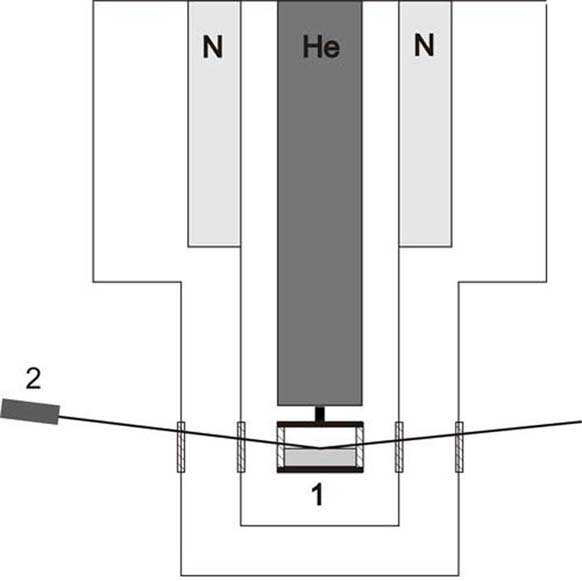
\includegraphics [scale=0.2] {article1/kriostat.jpg} \\ а)
  \end{minipage}
 \hfill
  \begin{minipage}[ht]{0.48\linewidth}
  \center
  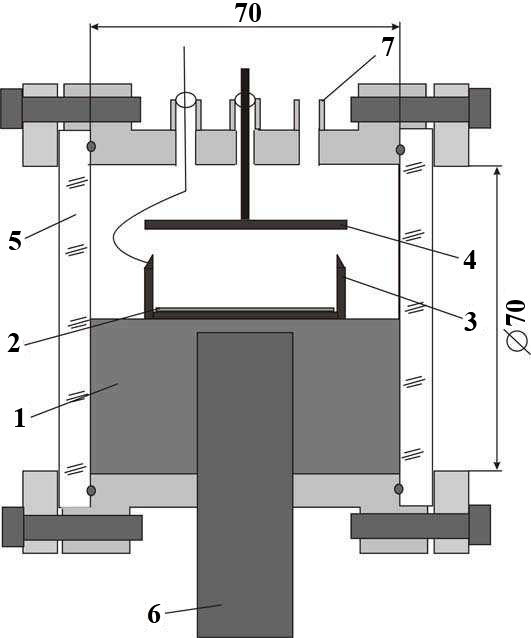
\includegraphics [scale=0.2] {article1/cell.jpg} \\ б)
   \end{minipage}
   \caption{  
   %а) Схематичная конструкция криостата. 1 – экспериментальная ячейка, 2 – лазер.   
  %б) Схематичная конструкция экспериментальной ячейки.  1 – текстолитовый брусок, 2 – радиоактивная мишень, 3 – медный контейнер, 4 – верхняя обкладка конденсатора, 5 – кварцевое окно, 6 - медный хладопровод, 7 – капилляр для набора водорода.
а) Конструкция криостата. б) Конструкция экспериментальной ячейки.
  } 
 
\label{img:cryostat} 
 
\end{figure}

Экспериментальная установка состоит из гелиевого криостата (рис.~\ref{img:cryostat}а), в вакуумной полости которого расположена оптическая ячейка (рис.~\ref{img:cryostat}б), системы возбуждения колебаний на поверхности жидкого водорода и оптической системы их регистрации. Жидкий водород конденсируется в цилиндрическую ячейку диаметром 60 мм и глубиной 6 мм. Радиоактивная мишень (молибденовая пластина, покрытая слоем тритида титана), расположенная на дне стакана, ионизирует жидкий водород. Колебания на заряженной поверхности жидкости возбуждаются переменным электрическим полем. В экспериментах в качестве переменного возбуждающего напряжения были использованы низкочастотные случайные сигналы, сосредоточенные в полосе частот 39-103 Гц.  Средний квадрат возбуждающего напряжения менялся от $V_p$ = 0 В, т.е. отсутствие накачки, до $V_p$ = 30 В


Для регистрации волн на поверхности жидкости использовался метод отраженного лазерного луча \cite{Brazhnikov_IET} в режиме "широкого"{} луча. При этом квадрат Фурье образа сигнала, принятого фотодетектором после отражения от поверхности жидкости, $P_\omega^2$ будет пропорционален Фурье образу парной корреляционной функции отклонения поверхности от положения равновесия $I(\omega)$.

\begin{figure}[ht] 
 \begin{minipage}[ht]{0.48\linewidth}
   \center
   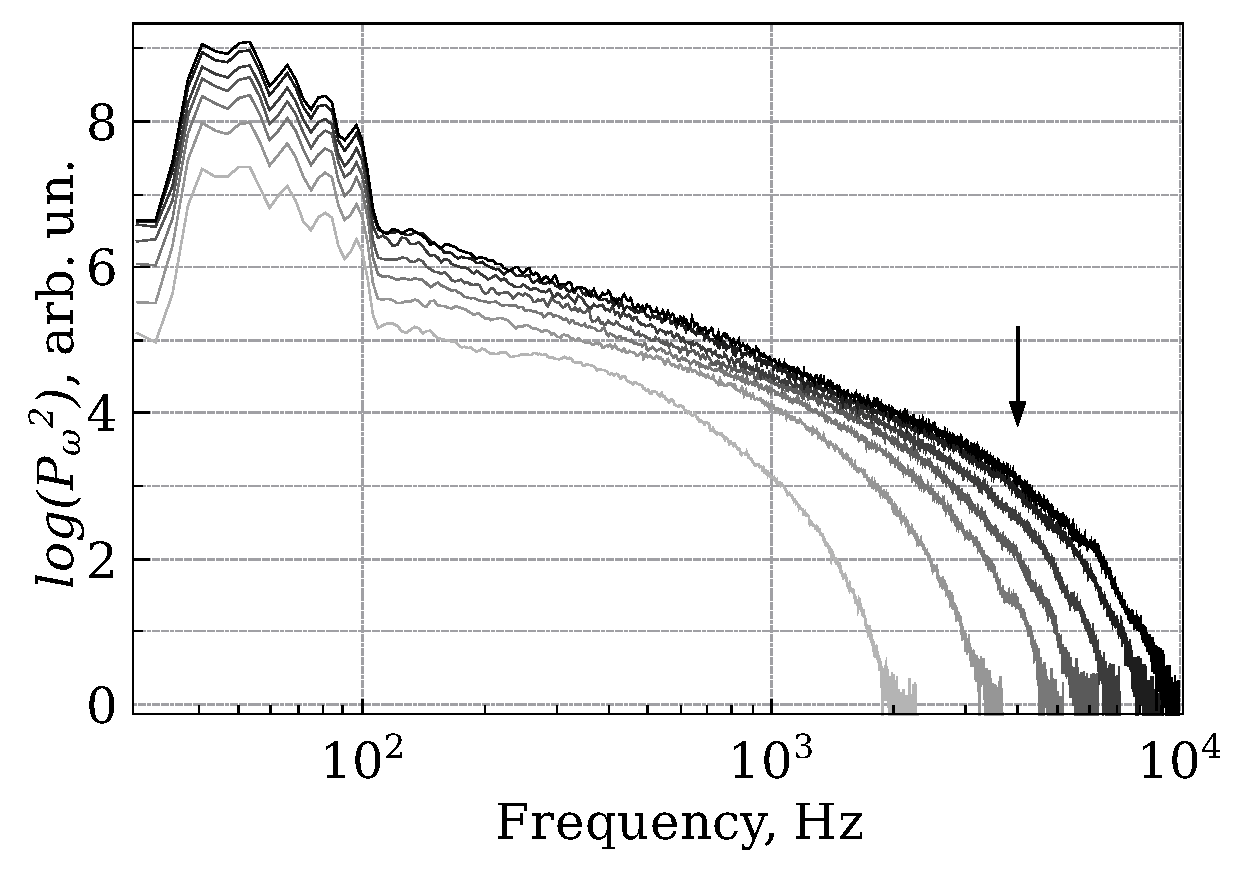
\includegraphics [scale=.275] {article1/spectra_dlog.eps} \\ а)
 \end{minipage}
 \hfill
 \begin{minipage}[ht]{0.48\linewidth}
   \center
   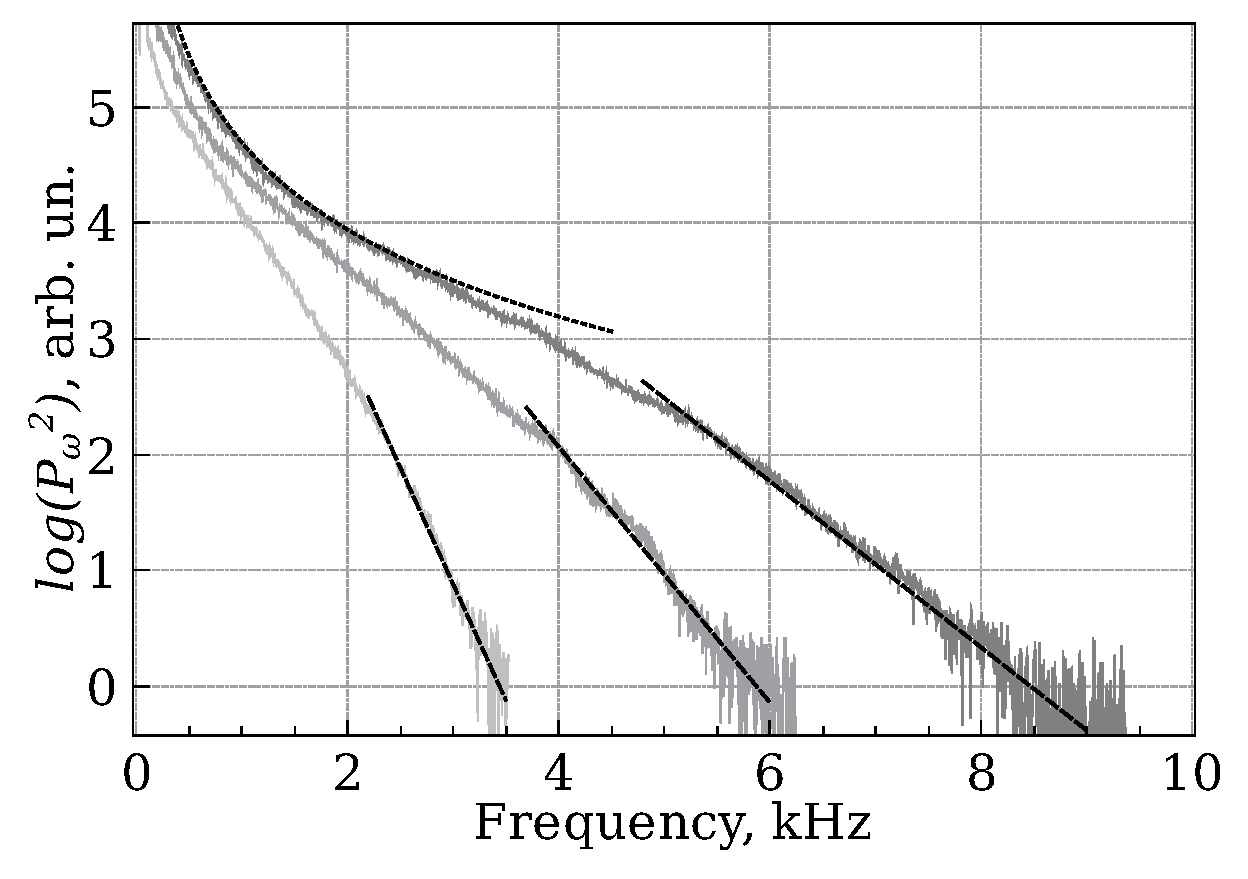
\includegraphics [scale=0.275] {article1/spectra_log.eps} \\ б)
\end{minipage}

 \caption{а) Спектры поверхностных колебаний $P^2_\omega$, возбужденных случайной силой в частотном диапазоне 39-103 Гц при разных амплитудах возбуждающей силы. Среднеквадратичное значение возбуждающего напряжения $V_P$ меняется от 4 до 30 В. Более темные линии соответствуют большей силе накачки. Стрелкой показана высокочастотная граница инерционного интервала $\omega_b \approx 4$ кГц при накачке 30 В.
  б)Спектры $P^2_\omega$ для уровней накачки $V_p = 8$ В (светло серая линия), $16$ В (серая линия) и $26$ В (темно-серая линия) в полулогарифмическом масштабе. Линией из точек показан степенной закон $\sim \omega^{-2.8}$, пунктирной линией - подгонка функцией $ \sim e^{-\omega/\omega_d}$. $\omega_d$ примерно равен 0.2, 0.4 и 0.6 кГц для $V_p$ = 8, 16 и 26 В соответственно.} 
 \label{img:hydr_specrta_dlog} 
\end{figure}

На Фурье-спек­трах отраженной энергии лазерного луча $P_\omega^2$ при разных амплитудах воз­буждающей силы видно (см. рис.~\ref{img:hydr_specrta_dlog}а), что ширина инерционного интервала зависит от амплитуды накачки. Увеличение силы накачки приводит к уширению инерционного интервала, высокочастотная граница инерционного интервала $\omega_b$ смещается к высоким частотам. 



Турбулентные спектры, построенные в полулогарифмическом масштабе (см. рис.~\ref{img:hydr_specrta_dlog}б), показывают, что распределение энергии в диссипативной области близко к экспоненциальному $P_\omega^2 \sim e^{-\omega/ \omega_d}$, причем характерная частота $\omega_d$ растет с увеличение амплитуды.

%\begin{figure}[ht] 
% \center
% 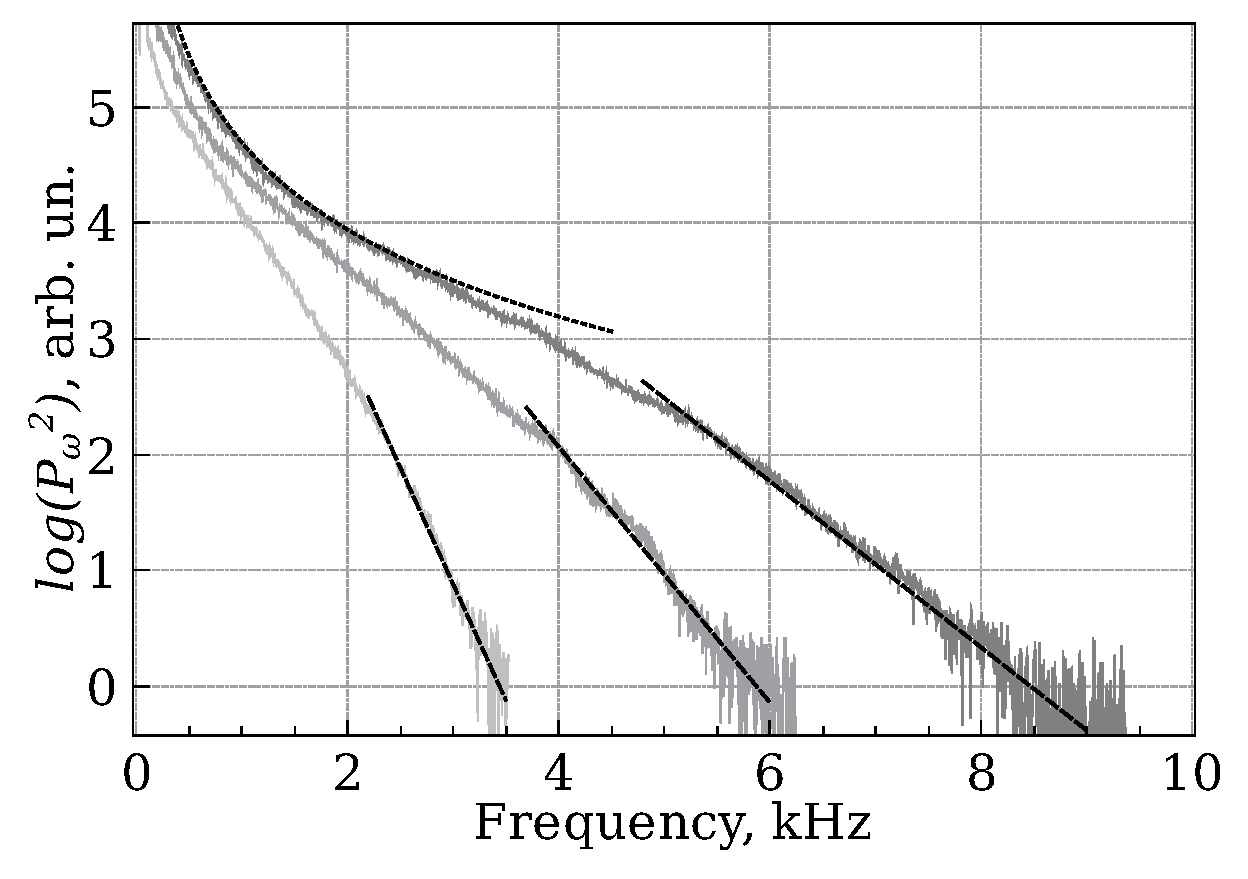
\includegraphics [scale=0.3] {article1/spectra_log.eps}
% \caption{Спектры $P^2_\omega$ для уровней накачки $V_p = 8$ В (светло серая линия), $16$ В (серая линия) и $26$ В (темно-серая линия) в полулогарифмическом масштабе. Линией из точек показан степенной закон $\sim \omega^{-2.8}$, пунктирной линией - подгонка функцией $ \sim e^{-\omega/\omega_d}$. $\omega_d$ примерно равен 0.2, 0.4 и 0.6 кГц для $V_p$ = 8, 16 и 26 В соответственно.} 
% \label{img:hydr_specrta_log} 
%\end{figure}

Для измерения уровня возбуждения использовался отклик поверхности $\eta_0$ , а именно абсолютное значение $P_\omega$ на частоте 53 Гц (положение максимума распределения $P_\omega^2$ внутри области накачки). Величина $\eta_0$ прямо пропорциональна средней высоте волны на той же самой частоте. На рис.~\ref{img:hydr_wd}  показано, что зависимость граничной частоты от значения амплитуды волны может быть описана степенным законом $\omega_d(\eta_0) \sim \eta_0^m$ со значение показателя $m = 0.85 \pm 0.05$, в то время как теория слабой волновой турбулентности предлагает значение $m = -12/5$. Стоит отметить, что подгонка экспоненциальных спектров с помощью "квазипланковского"{} распределения с малым ненулевым $s$ ($\vert s \vert \leq 2$) слабо влияет на полученный параметр $\omega_d$ (изменение менее 20\%). Эта поправка не изменит показатель степени $m$ в пределах погрешности.
\begin{figure}[ht] 
 \center
 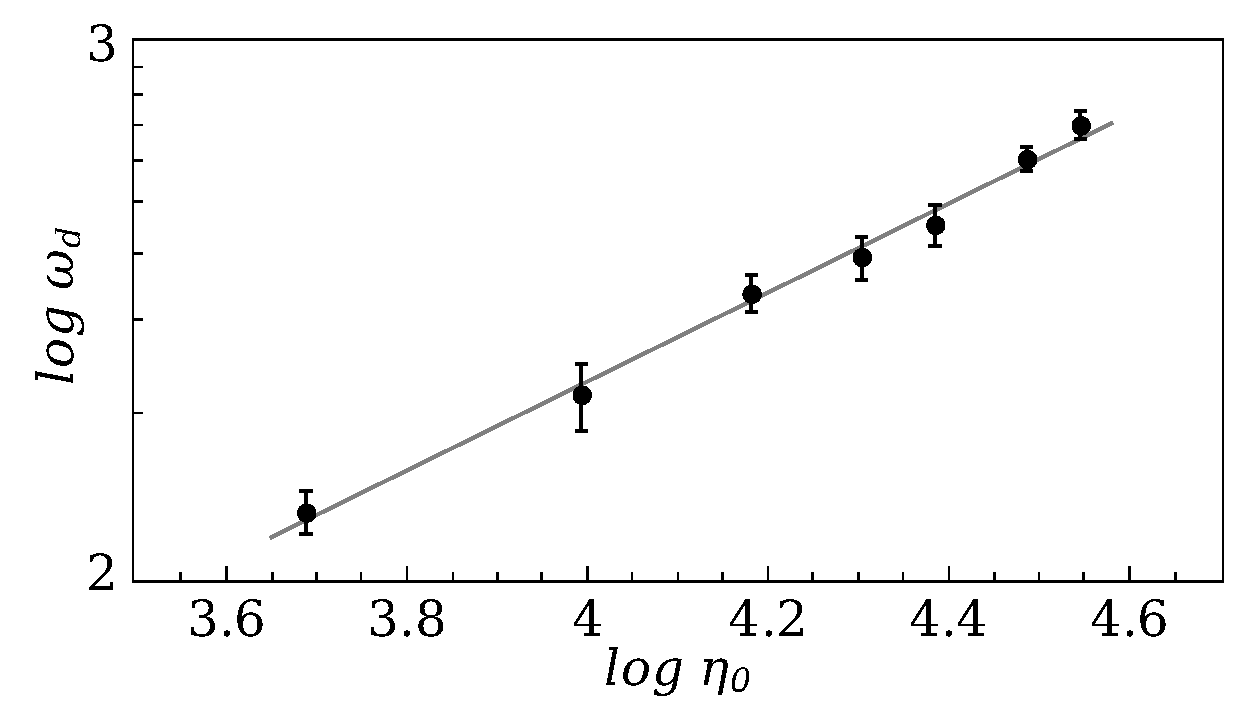
\includegraphics [scale=0.35] {article1/wd.eps}
 \caption{
 Зависимость частоты вязкого затухания диссипативной области $\omega_d$ (черные точки) от средней высоты низкочастотной волны $\eta_0$, сплошная линия - подгонка функцией $\eta_0^{0.85}$. }
 \label{img:hydr_wd} 
\end{figure}
Таким образом можно сделать выводы, что:

 - впервые наблюден переход от степенного спектра Колмогова-Захарова
в инерционном интервале к "квазипланковскому"{} распределению $\omega^{-s} e^{-\omega/\omega_d}$ в области диссипации энергии в турбулентном распределении системы капил­лярных волн;

- экспоненциальный спад в области диссипации $-\omega/ \omega_d \gg 1$ соответствует теоретическому ожиданию и качественно соответствует численным вычислениям \cite{Ryzhenkova1990}.
 
- граница вязкого затухания $\omega_d$ растет с увеличением амплитуды накачки и зависит от средней высоты волны $\eta_0$ на частоте накачки как $\omega_d \sim \eta_0^{0.85 \pm 0.05}$. Однако наблюденная зависимость отличается от теоретически ожидаемой, показатель степени почти в три раза больше предсказанного значе­ния.

\underline{\textbf{Вторая глава}} посвящена экспериментальному изучению особенностей распределения энергии в диссипативной области стационарного турбулентного спектра в системе капиллярных волн на поверхности воды, а также положению высокочастотной границы инерционного интервала в зависимости от амплитуды и типа накачки.

Экспериментальные ячейки имели форму стакана с кругом диаметром от 65 до 130 мм или прямоугольником со сторонами 49 $\times$ 50 мм в основании и глубиной 10 мм. Колебания на поверхности воды возбуждаются вертикальными колебаниями экспериментальной ячейки. Методика регистрации была такая же как в экспериментах с жидким водородом. Использовались следующие виды накачек: монохроматическая на резонансной частоте, узкополосная с шириной полосы около 1 Гц и широкополосная в диапазоне 30–50 Гц. Под амплитудой накачки А в случае монохроматического возбуждения понимается амплитуда электрического сигнала, подаваемого на виброплатформу. В случае узкополосной или широкополосной накачки за амплитуду А принимается среднеквадратичное значение электрического сигнала, подаваемого на виброплатформу.

\begin{figure}[ht]
 \begin{minipage}[ht]{0.49\linewidth}
 \center{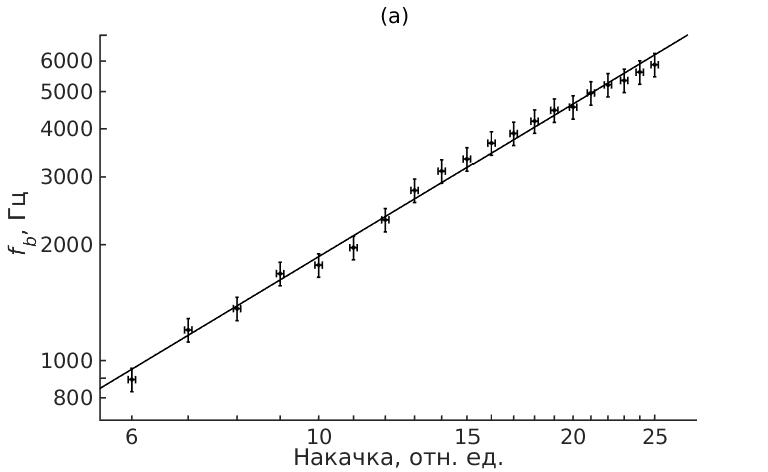
\includegraphics[width=1\linewidth]{article2/pic_06a.jpg} \\ а)}
 \end{minipage}
 \hfill
 \begin{minipage}[ht]{0.49\linewidth}
 \center{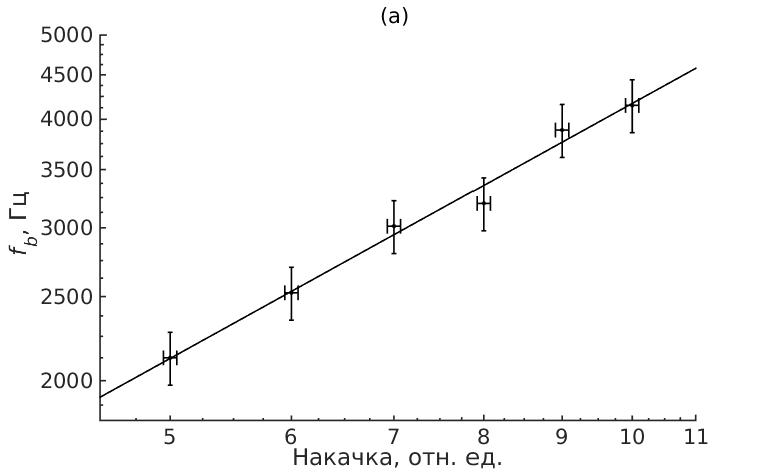
\includegraphics[width=1\linewidth]{article2/pic_07a.jpg} \\ б)}
 \end{minipage}
 \caption{Зависимость высокочастотного края инерционного интервала $f_b$ от амплитуды возбуждающей силы в цилиндрических ячейках диаметром 65 мм, при а) монохроматической накачке на частоте $f_p$ = 45.5 Гц. Прямая линия соответствует степенной зависимости частоты от амплитуды накачки с показателем степени $\beta = 1.32$
 б) широкополосной накачки в интервале 30–50 Гц. Прямая линия соответствует степенной зависимости частоты от амплитуды накачки с показателем степени $\beta = 0.97$}

 \label{img:water_fb_65} 
\end{figure}
Экспериментальное исследование дает степенную зависимость положения границы инерционного интервала в зависимости от амплитуды накачки для разных типов накачки $f_b \sim A^\beta$ (см. рис.~\ref{img:water_fb_65}).

 Так же степенным образом зависит от амплитуды накачки характерная частота в показателе экспоненты, описывающей затухание распределения энергии в диссипативной области турбулентного спектра $f_d \sim A^\beta$ (см. рис.~\ref{img:water_fd_65}).



При монохроматической накачке получаются зависимости: $f_b \sim A^{1.23 \pm 0.10}$,  $f_d \sim A^{1.28 \pm 0.10}$. Видно, что показатели степени близки к теоретическому значению для монохроматической накачки $\beta = -4/3$.

Для широкополосной накачки получаются зависимости: $f_b \sim A^{0.96 \pm 0.02}$,  $f_d \sim A^{1.13 \pm 0.00}$, отличающиеся от теоретического значению $\beta = -12/5$.

Таким образом можно сделать выводы:

-экспериментально показано, что при возбуждении турбулентного состояния на поверхности воды монохроматической или широкополосной накачкой частота высокочастотного края инерционного интервала и характерная частота вязкого затухания каскада $P_\omega^2$ в диссипативной области отличаются в несколько раз и качественно одинаково повышаются с ростом амплитуды накачки по степенному закону с показателем степени, близким к теоретически оцененному значению для монохроматического возбуждения;

- в случае широкополосной накачки наблюдается значительное расхождение между экспериментальными и теоретически оцененными значениями показателя $\beta$; 

- показано, что значения показателя степени слабо зависит от геометрии экспериментальной ячейки.

\begin{figure}[ht]
 \begin{minipage}[ht]{0.49\linewidth}
 \center{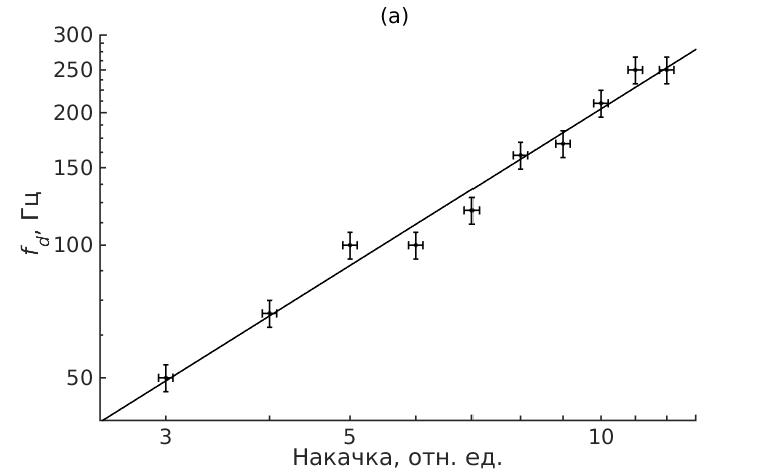
\includegraphics[width=1\linewidth]{article2/pic_09a.jpg} \\ а)}
 \end{minipage}
 \hfill
 \begin{minipage}[ht]{0.49\linewidth}
 \center{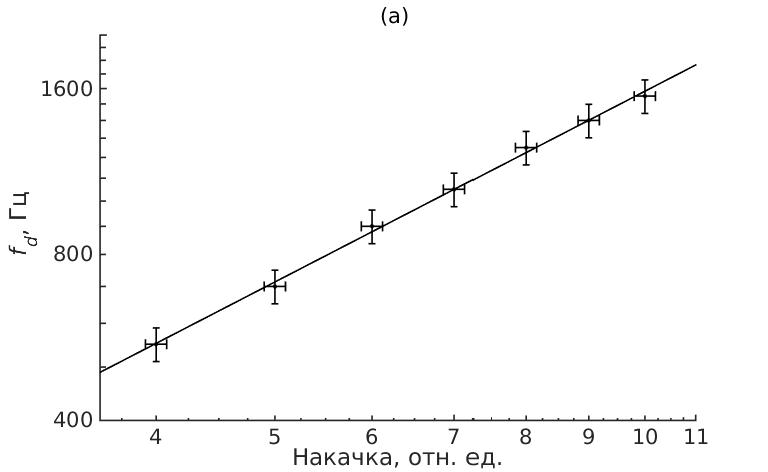
\includegraphics[width=1\linewidth]{article2/pic_11a.jpg} \\ б)}
 \end{minipage}
 \caption{Зависимость характерной частоты $f_d$ от амплитуды возбуждающей силы в ячейке диаметром 65 мм при а) монохроматической накачке на частоте 45.5 Гц. Прямая линия соответствует степенной зависимости частоты от амплитуды накачки с показателем степени $\beta = 1.18$.
 б) широкополосной накачке на частотах от 30 до 50 Гц в ячейке диаметром 65; Прямая линия соответствует степенной зависимости частоты от амплитуды накачки с показателем степени $\beta = 1.15$.}
 \label{img:water_fd_65} 
\end{figure}


\underline{\textbf{Третья глава}} посвящена исследованию генерации вихревого движения из-за взаимодействия нелинейных капиллярных волн, распространяющихся под углом друг к другу, на поверхности воды.

Экспериментальная установка
%(см. рис.~\ref{img:setup50})
 состоит из виброплатформы, на которой установлена ячейка цилиндрической (диаметр 65 мм) или прямоугольной (49 $\times$ 50 мм$^2$) формы глубиной 10 мм. В экспериментальную ячейку налита дистиллированная воды. Для декорирования вихревного движения на поверхность воды насыпаны полые алюмосиликатные микросферы или частички полиамида PA-12. Над ячейкой расположена камера, которая снимает движение частичек на поверхности воды. Полученное видео разбивается на кадры и для каждой последовательной пары кадров с помощью пакета PIVlab для Matlab \cite{PIVlab} вычисляется поле скорости на поверхности жидкости.

%\begin{figure}[ht] 
% \center
% 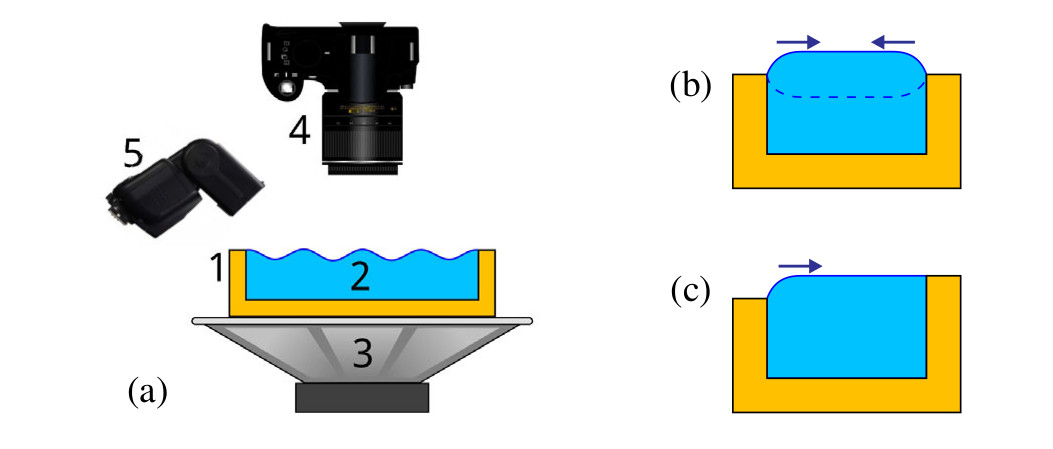
\includegraphics [scale=1] {article4/pic_01.jpg}
% \caption{Экспериментальная установка для регистрации вихревых движений на поверхности воды. а) Схема установки: 1 - ячейка, 2 - вода, 3 - виброплатформа, 4 - фотоаппарат, 5 - фотовспышка. b) Вогнутый или выпуклый мениск формируется на краю стенок в зависимости от количества воды, используемой для заполнения сосуда. с) Конфигурация водяного мениска в квадратной ячейке, имеющей стенки разной высоты, предназначенная для подавления генерации волн от пары соседних стенок. Стрелки показывают направление распространения волны.} 
%  \label{img:setup50} 
%\end{figure}
При возбуждении волн радиальной моды в цилиндрической ячейке вихрей на поверхности воды не возникает (см рис.~\ref{img:vort_st}а). Изменение симметрии ячейки путем добавления двух столбушков приводит к появлению вихревой структуры  (см. рис.~\ref{img:vort_st}б). При возбуждении угловой моды в цилиндрической ячейке или двух перпендикулярных волн в прямоугольной ячейке на поверхности воды также возникает вихревая структура, напоминающая структуру волн (см. рис.~\ref{img:vort_chess}а). Таким образом можно сделать предположение, что вихревое движение возникает за счет взаимодействия волн, распространяющихся под углом друг к другу.

\begin{figure}[ht]
 \begin{minipage}[ht]{0.49\linewidth}
 \center{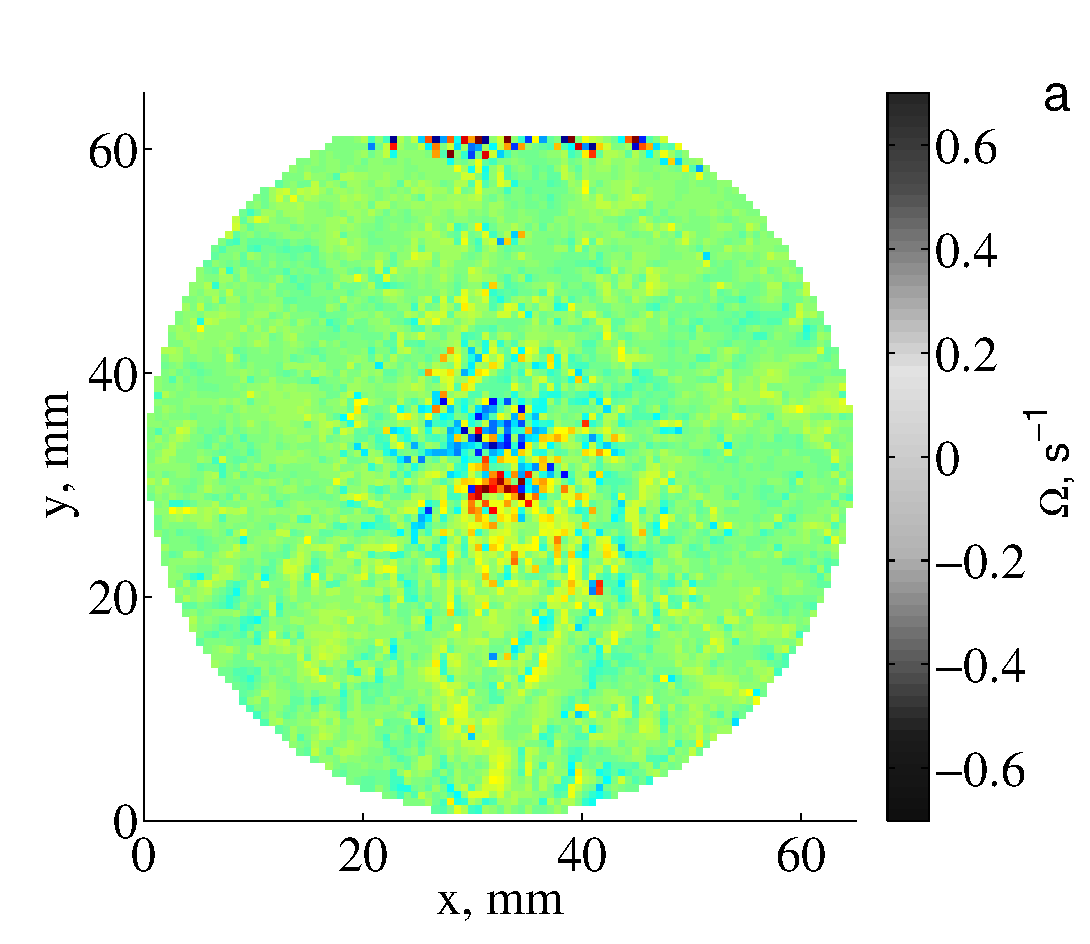
\includegraphics[width=1\linewidth]{article3/pic_06a.eps} \\ а)}
 \end{minipage}
 \hfill
 \begin{minipage}[ht]{0.49\linewidth}
 \center{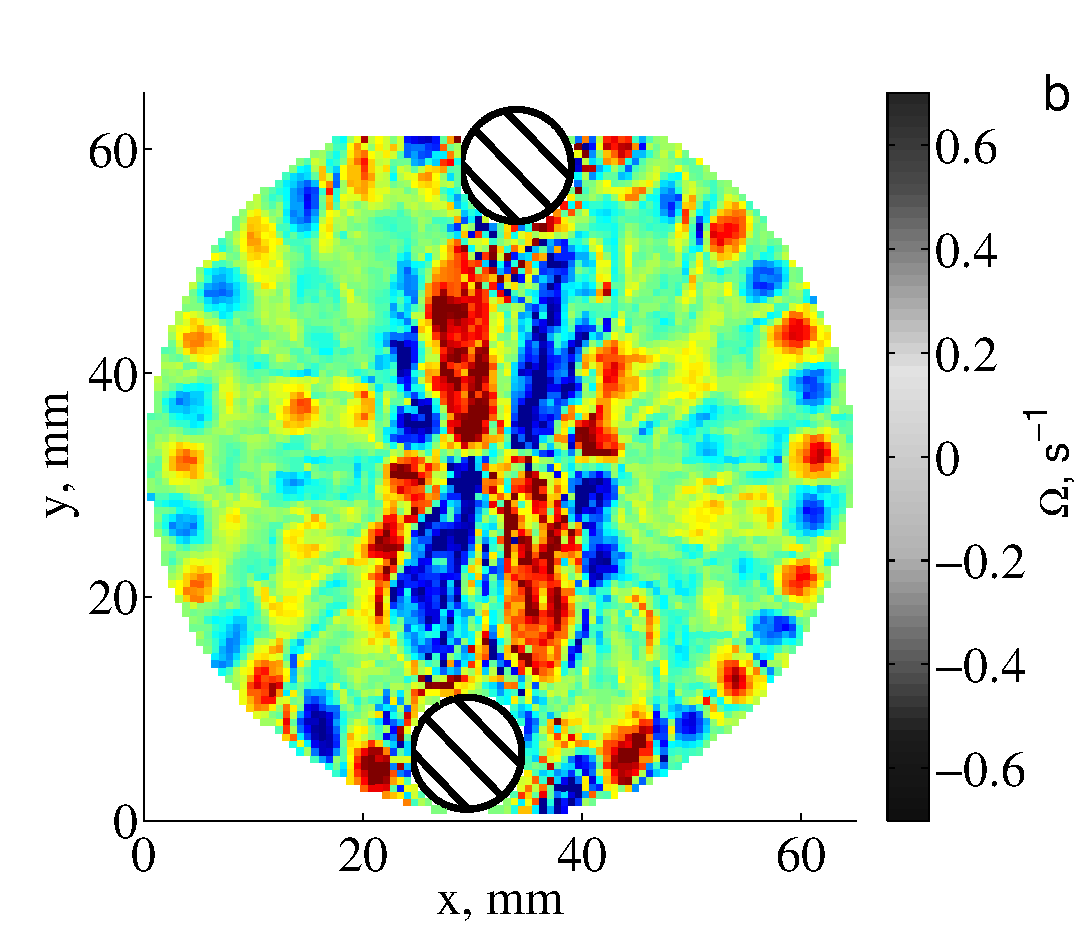
\includegraphics[width=1\linewidth]{article3/pic_06b.eps} \\ б)}
 \end{minipage}
 \caption{Поле завихренности $\Omega$ в цилиндрическом сосуде, в котором установлены два пластиковых столбика. На вставке – завихренность до установки столбиков. Цветовая шкала для завихренности общая.}
 \label{img:vort_st} 
\end{figure}

В работе \cite{F6} была построена теоретическая модель генерации вихревого движения в случае взаимно перпендикулярных стоячих волн и в случае взаимно перпендикулярных бегущих волн.

\begin{figure}[ht] 
 \begin{minipage}[ht]{0.49\linewidth}
  \center
  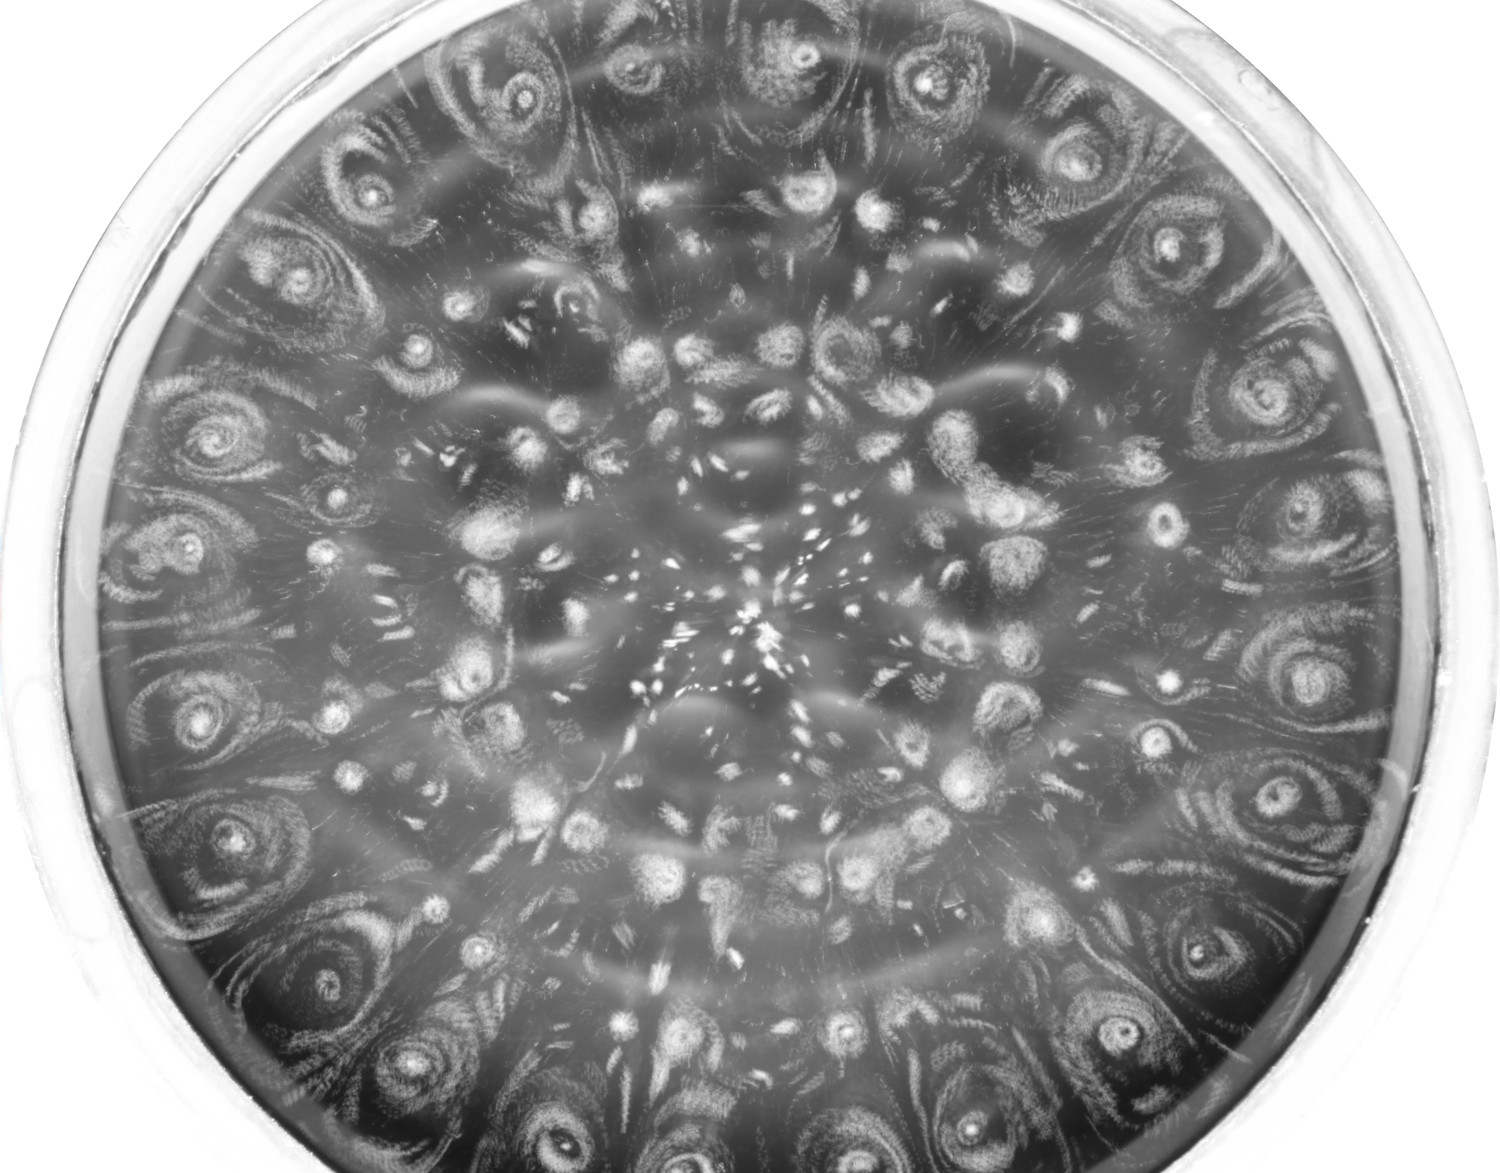
\includegraphics [scale=.38] {article4/pic_02.eps}
 \end{minipage}
 \hfill
 \begin{minipage}[ht]{0.49\linewidth}
  \center
  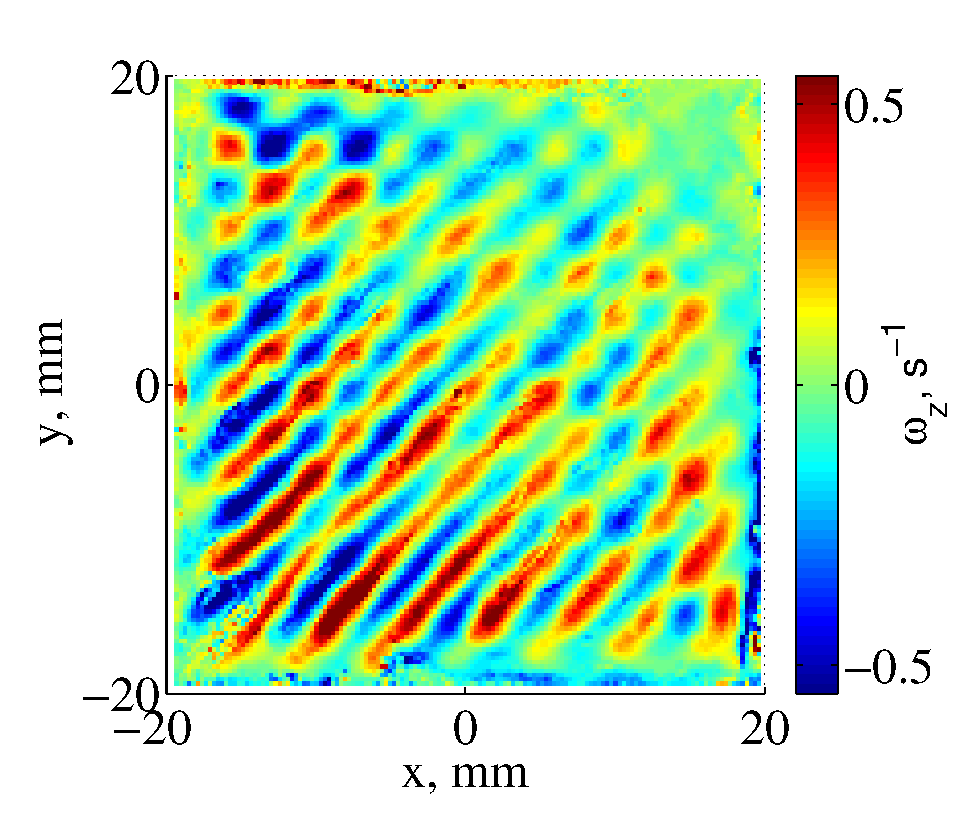
\includegraphics [scale=.38] {article4/pic_03.eps}
 \end{minipage}  
 \caption{а) Завихренность в ячейке 50 x 49 мм$^2$ при возбуждении поверхностных волн с частотой 42.7 Гц. Наблюдается шахматноподобный паттерн поля завихренности соответствующий теоретическому выражению (\ref{eq:vortStand}). Периоды решетки в $X$ и $Y$ направлениях равны длине волны.
 б) Завихренность в ячейке 40 х 40 мм $^2$ при возбуждении поверхностных волн с частотой 54 Гц. Две стенки ячейки соответствующие левой и нижней части рисунка немного ниже, чем остальные станки. Уровень воды скорректирован, чтобы в основном возникало две бегущие волны от более низких стенок. Знакопеременные полосы положительной и отрицательной завихренности, направленные параллельно диагонали квадратной ячейки, согласуются с теоретическим выражением (\ref{eq:vortRun}).} 
 \label{img:vort_chess} 
\end{figure}

В первом случае теоретическая модель построена для двух стоячих волн, описываемых уравнением:

\begin{equation}
\label{eq:waveStand}
h(x, y, t) = H_1 sin(kx)cos(\omega t)+H_2 sin(ky)cos(\omega t+ \phi),
\end{equation}
где $\phi$ разность фаз между стоячими волнами в разных направлениях.

Согласно предсказанию построенной модели завихренность на поверхности жидкости в стационарном режиме будет описываться выражением:

\begin{equation}
\label{eq:vortStand}
\Omega = -(1 + \sqrt{2}) H_1 H_2 \omega k^2 sin(kx)sin(ky) sin \phi
\end{equation}

Эксперимент по генерации завихренности на поверхности воды в прямоугольной ячейке размером 49 $\times$ 50 мм$^2$ показывает пространственное распределение завихренности качественно совпадающее с формулой (\ref{eq:vortStand}) (см. рис.~\ref{img:vort_chess}а). 


Серия экспериментов, проведенных при разном уровне накачки, показывает, что амплитуда завихренности решетки вихрей в зависит от амплитуды волны квадратичным образом (рис.~\ref{img:vort_ampl}), что хорошо согласуется с формулой (\ref{eq:vortStand}).

\begin{figure}[ht] 
 \center
 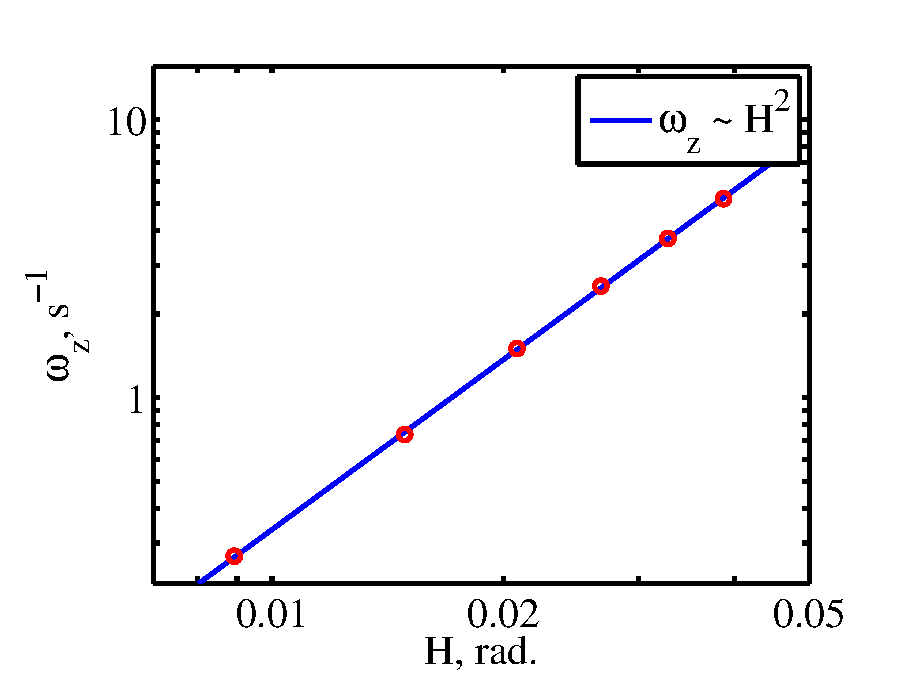
\includegraphics [scale=.35] {article4/pic_04.eps}
 \caption{Амплитуда завихренности для различных амплитуд накачки в ячейке 50 x 49 мм$^2$, где возбуждаются поверхностные волны с частотой 42.7 Гц, построенная в зависимости от амплитуды накачки. Линия соответствует зависимости $\Omega \sim H^2$.} 
 \label{img:vort_ampl} 
\end{figure}

Так же теоретическая модель построена для двух перпендикулярных бегущих волн, описываемых уравнением:

\begin{equation}
\label{eq:waveRun}
h(x, y, t) = H_1 sin(kx-\omega t)+H_2 sin(ky-\omega t)
\end{equation}

В этом случае завихренность на поверхности жидкости в стационарном режиме будет описываться выражением:

\begin{equation}
 \label{eq:vortRun}
\Omega = -(1 + \sqrt{2})H_1 H_2 \omega k^2 sin(kx-ky)
\end{equation}
Эксперимент по генерации завихренности на поверхности воды в квадратной ячейке размером 40 $\times$ 40 мм$^2$ показывает пространственное распределение завихренности качественно совпадающее с формулой (\ref{eq:vortRun}) (см. рис.~\ref{img:vort_chess}б). 

Таким образом можно сделать выводы:

 - открыт новый механизм генерации поверхностной завихренности, связан­ный с взаимодействием нелинейных поверхностных волн в тонком вязким под­слоем;

 - экспериментально наблюдена квадратичная зависимость модуля завих­ренности от угловой амплитуды волны;
 
 - наблюденные экспериментальные рас­пределения вихревого движения, генерируемого взаимно перпендикулярными как стоячими, так и бегущими волнами, качественно хорошо согласуются с тео­ретической моделью.


%Увеличивая амплитуду вертикальных колебаний ячейки можно достичь порога неустойчивости Фарадея. Значительно выше порога, поверхностные вол­ны весьма интенсивны, что приводит к интенсивным вихревым движениям по­верхности жидкости, для которых угловая амплитуда приближается к 1. Тогда взаимодействие вихревых движений друг с другом становится значительным [48], что приводит, в частности, к образованию каскада энергии [27]. Результа­ты наших теоретических и экспериментальных исследований позволяют лучше понять это явление и разработать количественную основу для него.

\underline{\textbf{Четвертая глава}} посвящена исследованию генерации вихревого движения из-за взаимодействия нелинейных гравитационных волн, распространяющихся под углом друг к другу, на поверхности воды.

\begin{figure}[ht]
 \begin{minipage}[ht]{0.49\linewidth}
 \center{\includegraphics[width=.82\linewidth]{article5/pic_02a.eps} \\ а)}
 \end{minipage}
 \hfill
 \begin{minipage}[ht]{0.49\linewidth}
 \center{\includegraphics[width=1\linewidth]{article5/pic_02b.eps} \\ б)}
 \end{minipage}
 \caption{а) Треки полиамидных частиц на поверхности воды при накачке двумя плунжерами на частоте 3\,Гц с угловой амплитудой волны в центре ванны $\mu = 0.035$ рад. б) Распределение завихренности на поверхности воды при накачке двумя плунжерами на частоте 3\,Гц. Разность фаз $\psi = 90^\circ$.}
 \label{img:vort_3Hz} 
\end{figure}
 
Экспериментальная установка состоит из ванны размером 70 $\times$ 70 см$^2$, заполненной дистиллированной водой. Глубина воды составляет 10 см. Волны на поверхности воды возбуждаются волнопродукторами - двумя перпендикулярными плунжерами совершающими вертикальные колебания по действием приводов плунжеров. В качестве плунжеров используются горизонтальные стальные полые трубки, запаянные с концов, полупогруженные в воду. Приводами плунжеров служат сабвуферы TS-W254R фирмы Pioneer номинальной мощностью 250 Вт. 


Для визуализации вихревого движения на поверхность воды насыпан порошок полиамида PA-12. Камера Canon 70D, расположенная над ванной, регистрирует движение частичек полиамида.
За счет того, что плунжеры не связаны друг с другом физически, можно устанавливать произвольную разность фаз между ними.

В экспериментах использовалась монохроматическая накачка на частотах 3,4,6 Гц.

При накачке на частоте 3 Гц (длина волны 17.5 см), на поверхности воды хорошо видна решетка вихрей с характерным размером вихря около 8 см (см рис.~\ref{img:vort_3Hz}а). Пространственное распределение завихренности в решетки вихрей, возбужденной на поверхности воды, соответствует теоретической модели.

Серия экспериментов проведенных при разном уровне накачки показывает что амплитуда завихренности решетки вихрей в зависит от амплитуды волны квадратичным образом (рис.~\ref{img:ampl_phase}а), что хорошо согласуется с формулой (\ref{eq:vortStand}).
\begin{figure}[ht]
 \begin{minipage}[ht]{0.48\linewidth}
 \center{\includegraphics[width=1\linewidth]{article5/pic_03a.eps} \\ а)}
 \end{minipage}
 \hfill
 \begin{minipage}[ht]{0.48\linewidth}
 \center{\includegraphics[width=1\linewidth]{article5/pic_03b.eps} \\ б)}
 \end{minipage}
 \caption{а) Зависимость корня квадратного амплитуды завихренности $\sqrt{\Omega_0}$ на поверхности воды от угловой амплитуды волн $\mu$ при накачке двумя плунжерами на частоте 3\,Гц. Разность фаз $\psi=90^\circ$. б) Зависимость амплитуды завихренности $\Omega_0$ от разности фаз между синусоидальными сигналами, подаваемыми на волнопродукторы. Точки – эксперимент, сплошная кривая $\Omega_0 = \,0.183\, sin(\psi)$}
 \label{img:ampl_phase} 
\end{figure}
 
Эксперименты, проведенные при фиксированной амплитуде и меняющейся разности фаз в диапазоне от 0 до 180 градусов, показывают синусоидальную зависимость амплитуды решетки вихрей от амплитуды накачки (см. рис.~\ref{img:ampl_phase}б), что также хорошо согласуется с теоретической формулой (\ref{eq:vortStand}).

Однако при накачках на частотах 4 и 6 Гц на поверхности воды помимо решетки вихрей образуются крупномасштабные вихревые течения. Пример такого движения показан на рис.~\ref{img:vort_4Hz}а. На рис.~\ref{img:vort_4Hz}б показаны спектры энергии при накачке на частотах 3, 4 и 6 Гц. Видно, что при накачке на частотах 4 и 6 Гц в спектре появляются пики на малых волновых числах, что соответствует крупномасштабным течениям.
\begin{figure}[ht]
 \begin{minipage}[ht]{0.49\linewidth}
 \center{\includegraphics[scale=0.38]{article5/pic_04a.eps} \\ а)}
 \end{minipage}
 \hfill
 \begin{minipage}[ht]{0.49\linewidth}
 \center
 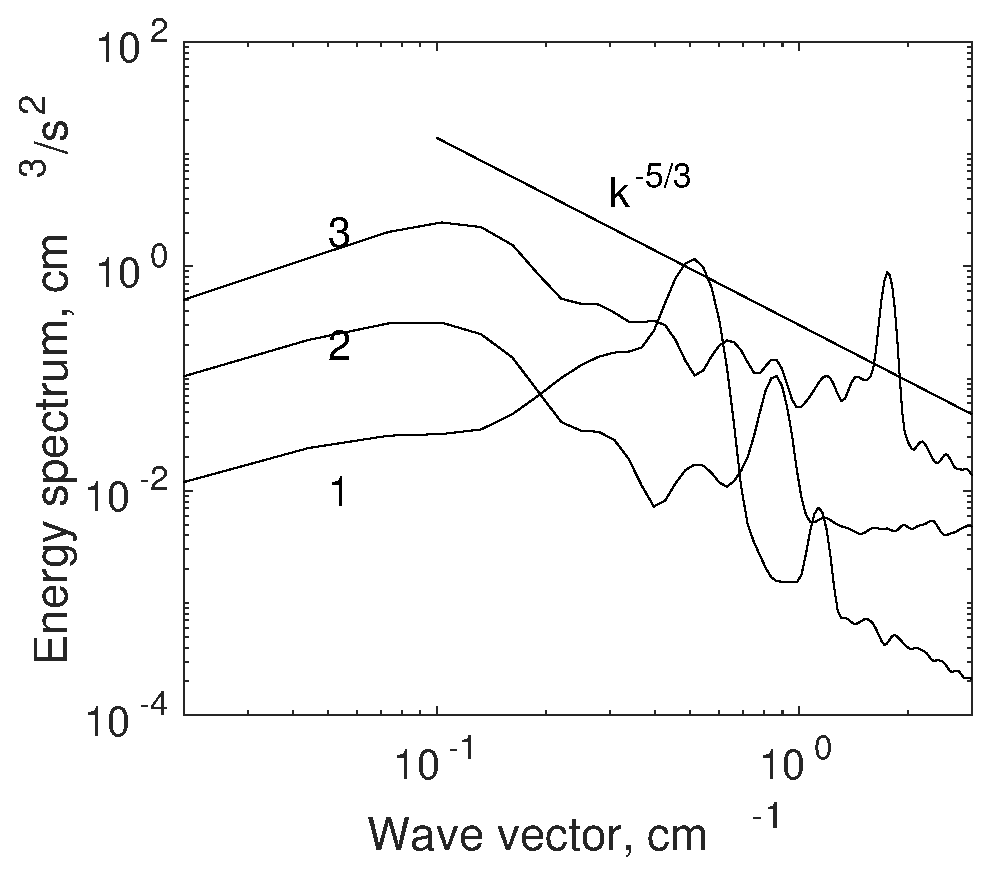
\includegraphics [scale=0.38] {article5/pic6_diss.eps}  \\ б)
 \end{minipage}
 \caption{а) Треки полиамидных частиц на поверхности воды при накачке двумя плунжерами на частоте 4\,Гц. Амплитуда волн на расстоянии 3\,см от плунжеров равна $H = 1.0 \pm 0.2$\,мм.
б) Распределение энергии $E(k)$ по волновому вектору при накачке двумя плунжерами на частоте 3\,Гц (кривая 1), 4\,Гц (кривая 2) и 6\,Гц (кривая 3).}
 \label{img:vort_4Hz} 
\end{figure}
Таким образом можно сделать выводы:

 - в данной работе впервые экспериментально показано, что завихренность,
формируемая на поверхности воды слабо нелинейными гравитационными волнами, зависит от разности их фаз и хорошо описывается выражениями, полу­ченными в работе \cite{F6}.

 - Амплитуда завихренности на поверхности квадратично зависит от амплитуды волн. Таким образом, модель генерации вихревого движения нелинейными волнами применима для описания завихренности на поверх­ности жидкости не только для волн капиллярного диапазона с длиной волны около 0.5 см, но и для гравитационных волн с длинами волн порядка 10 см.
 
 - Экспериментально наблюдена передача энергии из области накачки (масштаб решетки вихрей) в область больших масштабов. Механизм передачи энергии пока не установлен, требуются дополнительные исследования.
 
 \underline{\textbf{Пятая глава}} посвящена исследованию проникновению сгенерированной взаимодействием нелинейных волн решетки вихрей в объем жидкости.
 
Согласно построенной теоретической модели есть два механизма генерации вихревого движения волнами распространяющимися под углом друг к другу.

Первый, заключается в переносе жидкости в результате дрейфа Стокса. Согласно ему вихревое движение возникает сразу в каждой точке, где появляются волны, и исчезает сразу же как волны затухают или уходят из исследуемой области. Зависимость от глубины этой составляющей завихренности должна быть экспоненциальной:
\begin{equation}
 \label{eq:deepStocks}
\Omega_{St}(x,y,z) = e^{-2kz} sin \phi H_x(0) H_y(0) \omega k^2 sin(kx)sin(ky)
\end{equation}
Стоит также отметить, что из-за того, что дрейф Стокса наблюдается в лагран­жевых координатах, но не в эйлеровых, то это вихревое движение не имеет инерции и не существует отдельно от волн.  

Второй механизм отвечающий за генераций вихрей волновым движение описывает генерацию именно завихренности в эйлеровых координатах. Согласно ему завихренность возникает в результате нелинейного взаимодействия волн в тонком вязком приповерхностной подслое. Для волн частотой 3 Гц на поверхности воды его толщина будет равна $\delta = \sqrt{2 \nu / \omega} \sim 200 $ мкм \cite{FalkovichBook}. Завихренность из вязкого подслоя, проникает в объем диффузионным образом за счет вязкого трения между слоями жидкости. Таким образом, в стационарном режиме предсказывается так же экспоненциальное распределение завихренности по глубине, но отличным от формулы (\ref{eq:deepStocks}) показателем:
\begin{equation}
 \label{eq:deepEyler}
\Omega_N(x,y,z) = \sqrt{2}e^{-\sqrt{2}kz} sin \phi H_x(0) H_y(0) \omega k^2 sin(kx)sin(ky)
\end{equation}
Таким образом стоит ожидать, что завихренности будет зависеть от глубины как:
\begin{equation}
 \label{eq:deepFull}
\Omega(z) \sim \sqrt{2}e^{-\sqrt{2}kz} +  e^{-2kz}
\end{equation}

Регистрации завихренности в объеме жидкости производится с помощью методики "лазерного листа"{}. Для декорирования вихревого движения в объем вводятся частички полиамида PA-12, чья плотность близка к плотности воды. Частички подсвечивается лазерным листом, полученным пропусканием лазерного луча через цилиндрическую линзу диаметром 0.6 см, установленную вертикально. В работе использовался лазер MGL-H-532-500mW мощностью 0.5 Вт. После прохождения линзы лазерным лучом, он раскрывался в горизонтальный лазерный лист толщиной около 1 мм. Лазерный лист подсвечивает только те частицы в объеме жидкости, которые встречаются на его пути. Таким образом можно декорировать течения в объеме жидкости лежащие в плоскости лазерного листа. Видеосъемка частиц производилась камерой Canon 70D. В экспериментах использовалась монохроматическая накачка на частоте 3 Гц.
 

Пример получившего поля завихренность измеренного на глубине 0.5 см показан на рис.~\ref{img:underLong}а. Видно, что в объеме решетка сохраняет ту же форму, что и на поверхности жидкости.


\begin{figure}[ht]
 \begin{minipage}[ht]{0.64\linewidth}
  \center{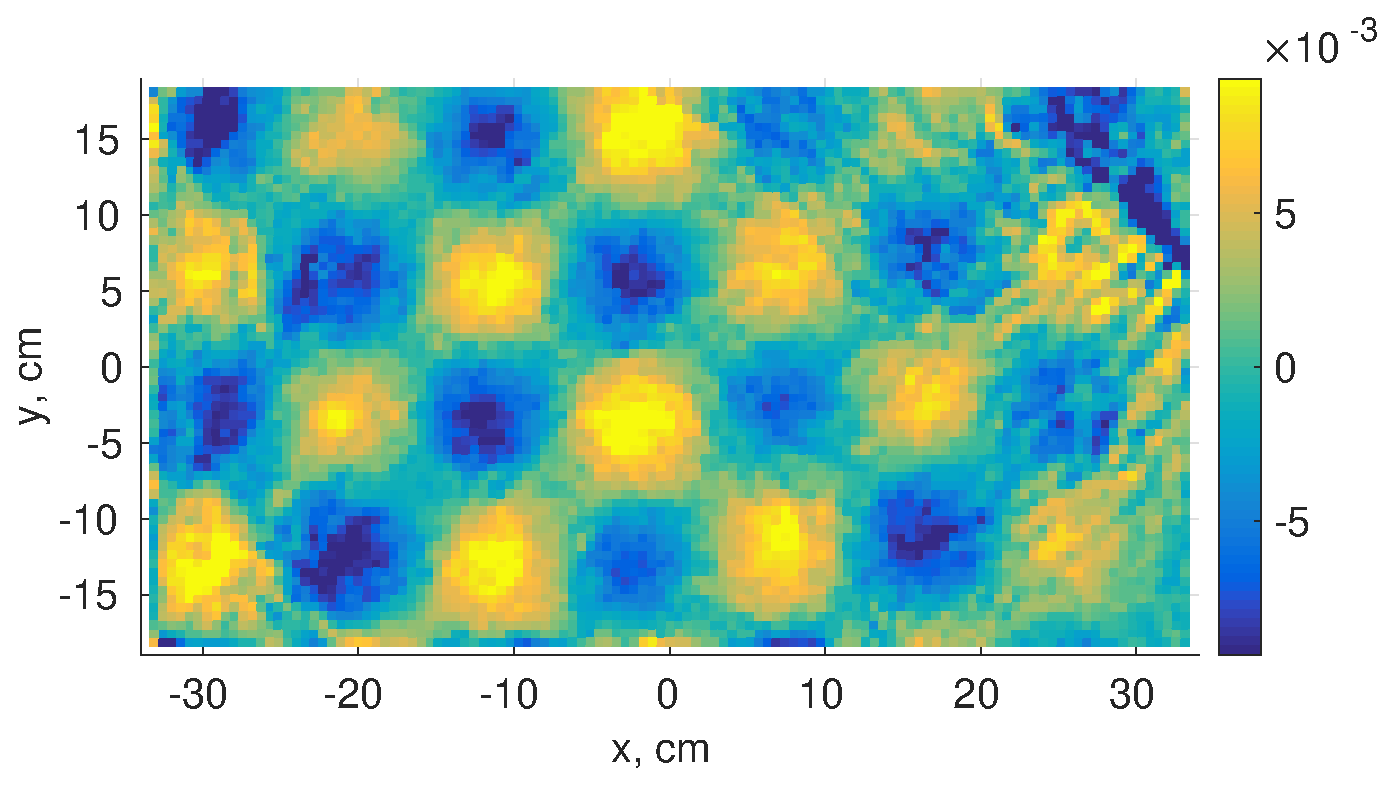
\includegraphics[width=.9\linewidth]{part6/vort0p5cm.eps} \\ а)}
 \end{minipage}
 \hfill
 \begin{minipage}[ht]{0.35\linewidth}
  \center
  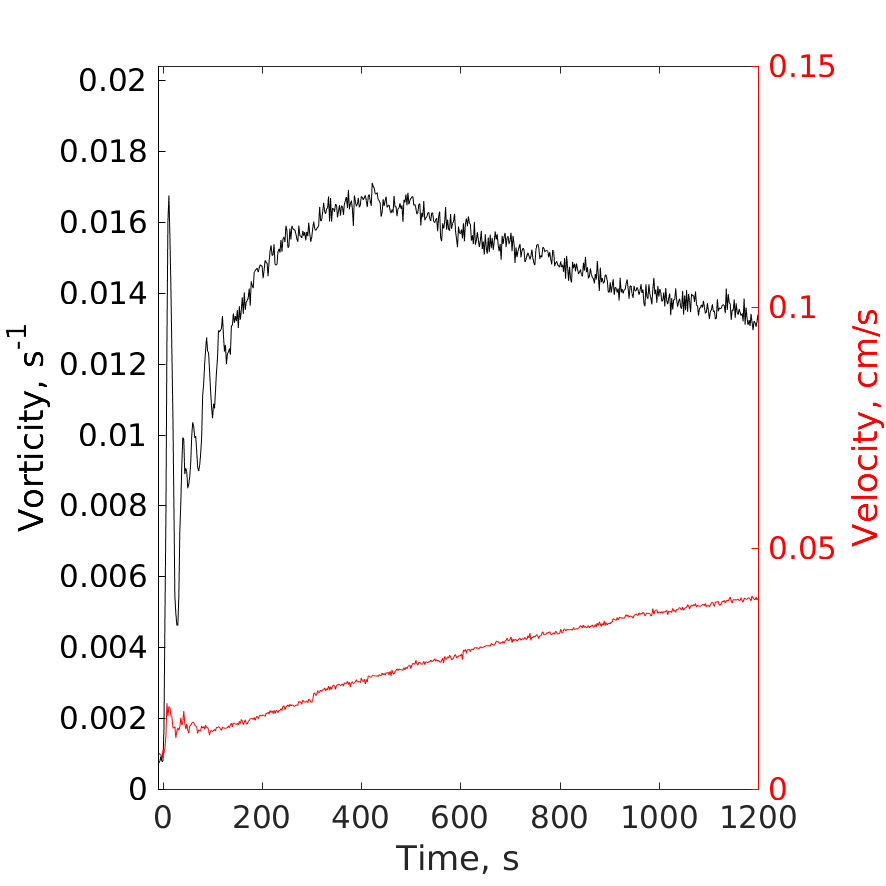
\includegraphics [width=1\linewidth]{part6/long_30mV_vel.jpg} \\ б)
 \end{minipage}

  \caption{а) Фрагмент 40х70 см$^2$ поля вертикальной завихренности в горизонтальном слое на глубине 0.5 см.
  б) Зависимость амплитуды завихренности решетки вихрей и скорости крупномасштабного течения от времени для амплитуд накачки  30 мВ на глубине 1 см.}
 \label{img:underLong} 
\end{figure}


\begin{figure}[ht]
  \center{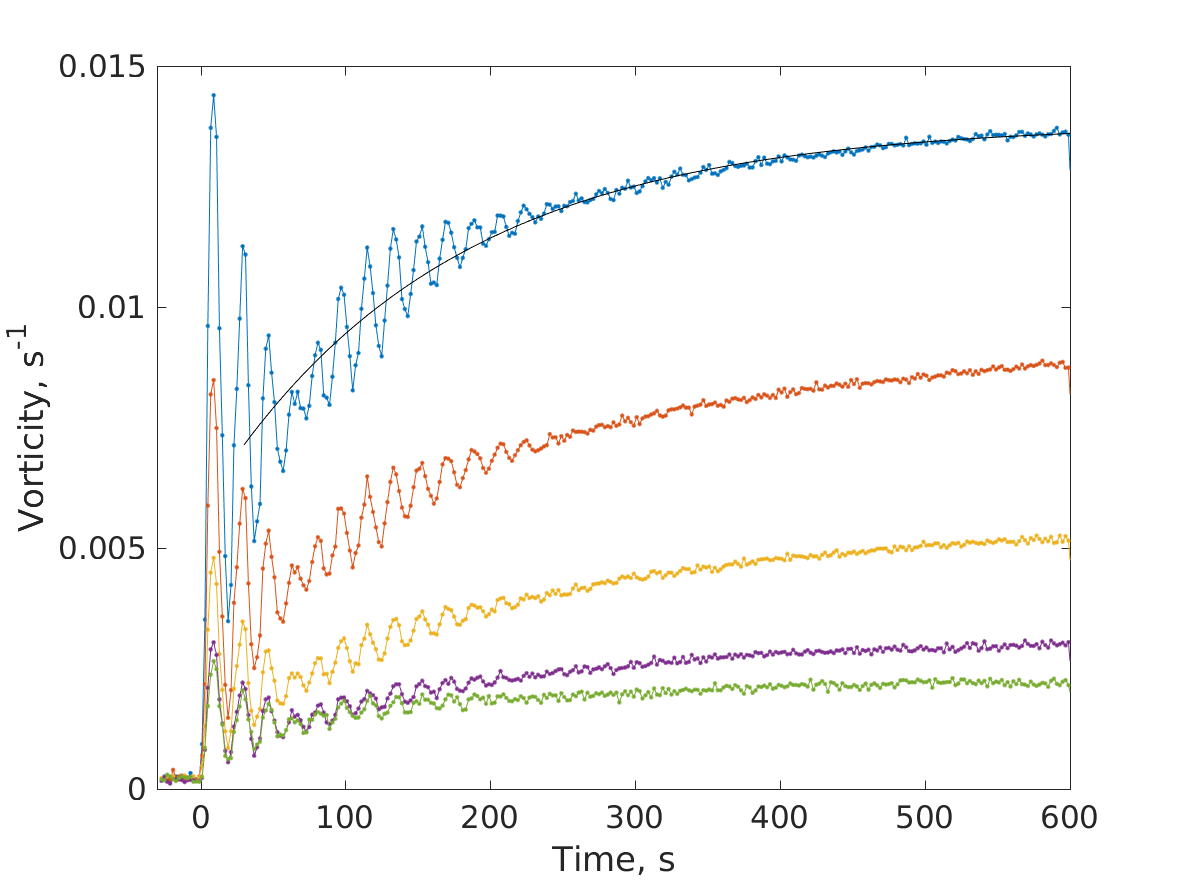
\includegraphics[width=.9\linewidth]{part6/5deeps.jpg} }

 \caption{Зависимость амплитуды завихренности решетки вихрей от времени, на глубинах 0.5~см, 1.25~см, 2.0~см, 2.75~см, 3.5~см. Черная кривая соответствует зависимости $1.4 \cdot 10^{-2} - 8 \cdot 10^{-3} e^{-t/165}$.}
 \label{img:5deeps} 
\end{figure}


На рисунке~\ref{img:5deeps} показана эволюция амплитуды решетки вихрей со временем после включения накачки. Пять кривых на рисунке соответствуют измерения на глубинах 0.5 см, 1.25 см, 2.0 см, 2.75 см, 3.5 см. Черной кривой показана зависимость $1.4 \cdot 10^{-2} - 8 \cdot 10^{-3} e^{-t/165}$.  Колебания завихренности на начальном участке объясняются колебанием амплитуд волн, связанными с переходными процессами. Т.е. на глубине 0.5 см завихренность росла с характерным временем 165 с. Оценка характерного времени роста завихренности для других глубин так же дают характерные времена около 200 с.


\begin{figure}[ht]
 \center
 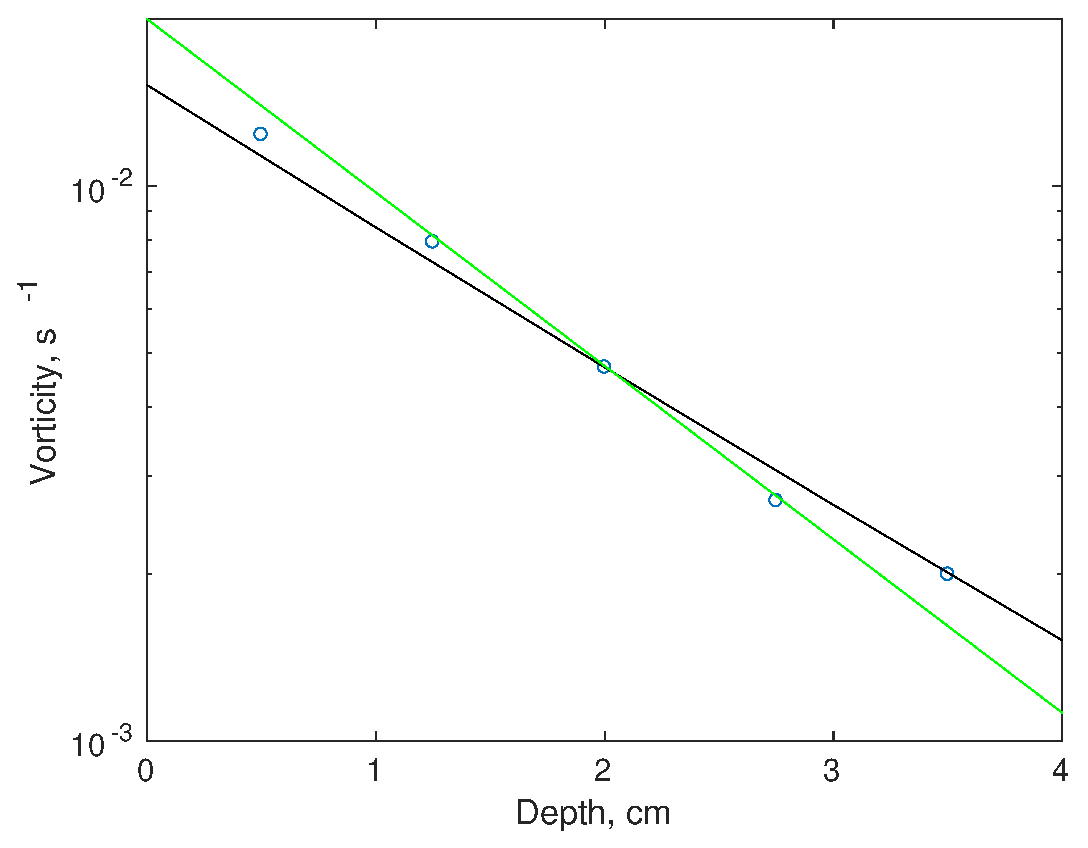
\includegraphics [width=.5\linewidth] {part6/depth.eps}
 \caption{Зависимость амплитуды завихренности решетки вихрей от глубины. Черная линия соответствует зависимости $6.3 \cdot 10^{-3} (e^{-2kh}+\sqrt{2}e^{-\sqrt{2}kh})$, зеленая прямая - $2 \cdot 10^{-2} e^{-2kh}$}
 \label{img:depth} 
\end{figure}

Также стоит отметить, что крупномасштабные вихревые течений, развивающиеся на поверхности воды сносят вихри и деформируют решетку завихренности. На рисунке~\ref{img:underLong}б показан график зависимости амплитуды решетки вихрей и средней скорости крупномасштабного течения от времени после включения накачки. На нем видно, что после 400-ой секунды завихренность решетки вихрей перестает расти и начинает уменьшаться. Начинает это происходить при характерной средней скорости крупномасштабного течения в $5 \cdot 10^{-3}$ см/с.

На рисунке~\ref{img:depth} показан график зависимости завихренности, усредненной в промежутке времени от 500 до 600 секунд после включения накачки, от глубины. Сплошные линии соответствуют зависимостям $e^{-2kh}+\sqrt{2}e^{-\sqrt{2}kh}$ и - $2 \cdot 10^{-2} e^{-2kh}$ , где k = 0.36~см$^{-1}$. Как видно из рисунка разброс экспериментальных точек не позволяют однозначно соотнести их с одной или другой экспоненциальной зависимостью. Стоит отметить, что снос завихренности решетки вихрей из-за развития крупномасштабных течений так же уменьшает значение завихренно­сти решетки вихрей, продиффундировавшей из вязкого подслоя. Этим, в свою очередь, можно объяснять расхождение экспериментальных данных с теоретической зависимостью

Таким образом можно сделать выводы:

-экспериментально показано, что распределение по глубине амплитуды завихренности решетки вихрей можно описать экспоненциальной зависимостью $e^{-2kh}$, где k — волновой вектор возбуждаемой решетки, а h — глубина слоя жидкости. 

-экспериментально оценено характерное время $\tau \approx 200$ с проникновения завихренности решетки вихрей из вязкого подслоя в объем. 

-экспериментально показано, что наличие крупномасштабных вихрей приводит к "сносу"{} завихренности, проникающей в объем из вязкого подслоя. Показано, что крупномасштабные течения с характерной скоростью $5 \cdot 10^{-3}$ см/c приводят к существенной деградации завихренности решетки вихрей с характерным размером вихря 8 см.


В \underline{\textbf{заключении}} приведены основные результаты работы, которые заключаются в следующем.

В диссертационной работе выполнены экспериментальные исследования капиллярной волновой турбулентности на поверхности жидкого водорода и воды, а так же исследования генерации вихревого движение на свободной поверхности жидкости волнами, движущимися под углом друг к другу.

1. Впервые наблюден переход от степенного распределения энергии в инерционном интервале спектра Колмогорова-Захарова к "квазипланковскому"{} распределению $\omega^{-s}e^{-\omega/\omega_d}$ в области диссипации для капиллярной турбулентности при накачке в полосе частот. Экспоненциальная зависимость энергии от частоты в области диссипации $\omega/\omega_d \gg 1$ соответствует теоретическому ожиданию и качественно соответствует численным вычислениям \cite{Ryzhenkova1990}. Граница вязкого затухания $\omega_d$ растет с увеличением амплитуды накачки и зависит от средней высоты волны $\eta_0$ на частоте накачки как $\omega_d \sim \eta^{0.85 \pm 0.05}$. Однако наблюденная зависимость отличается от теоретически ожидаемой, показатель степени почти в три раза меньше, чем предсказанное значение.

2. Экспериментально показано, что при возбуждении турбулентного состояния на поверхности воды монохроматической или широкополосной накачкой частота высокочастотного края инерционного интервала и характерная частота экспоненциального затухания энергии в диссипативной области отличаются в несколько раз друг от друга и качественно одинаково повышаются с ростом амплитуды накачки по степенному закону с показателем степени, близким к теоретически оцененному значению для случая монохроматического возбуждения. В случае возбуждения широкополосной накачкой наблюдается значительное расхождение между экспериментальными и теоретически оцененными значениями показателя $\beta$.

3. Открыт новый механизм генерации вихревого движения поверхностными волнами распространяющимися под углом друг к другу. Показано, что генерация вихревого движения на поверхности жидкости не является специфической чертой волн Фарадея.

4. Экспериментально подтверждена теоретическая модель генерации вихревого движения перпендикулярными волнами на поверхности воды как для капиллярных, так и для гравитационных волн. Экспериментально показано, что амплитуда завихренности решетки вихрей на поверхности воды квадратично зависит от амплитуды волн накачки, и зависит как $sin(\psi)$ от разности фаз $\psi$ между стоячими волнами в перпендикулярных направлениях. 

5. Экспериментально показано, что в объеме воды решетка вихрей сохраняет структуру и зависимость амплитуды завихренности от глубины близка к экспоненциальному закону $e^{-2kh}$, где k — волновой вектор возбуждаемой решетки, а h — глубина слоя жидкости. 
Экспериментально оценено характерное время проникновения завихренности решетки вихрей в объем при накачке двумя перпендикулярными волнами на частоте 3 Гц в 200 секунд.

6. Экспериментально показано, что наличие крупномасштабных вихрей приводит к сносу решетки вихрей. Оценены характерные скорости крупномасштабных течений приводящие к существенной деградации вихрей, формирующих решетку.


\clearpage 
\chapter*{Публикации автора}	% Добавляем его в оглавление
%
%
[F1] Brazhnikov M.Yu., Abdurakhimov L.V., Filatov S.V., Levchenko A.A., "Quasi-Planck"{} spectra of capillary turbulence on the surface of liquid hydrogen // JETP Lett. 2011.V. 93. P. 34.

[F2] Л.В. Абдурахимов, М.Ю. Бражников, А.А. Левченко, И.А. Ремизов, С.В. Филатов, "Турбулентный капиллярный каскад вблизи края инерционного интервала на поверхности квантовой жидкости"{}, Письма в ЖЭТФ, том 95 вып. 12, с. 751-760 (2012)

[F3] Л.В. Абдурахимов, М.Ю. Бражников, А.А. Левченко, И.А. Ремизов, С.В. Филатов, "Кинетическая и дискретная турбулентность на поверхности квантовой жидкости"{}, УФН, том 182, 8, с. 879 (2012)

[F4] С.В. Филатов, М.Ю. Бражников, А.А. Левченко, "Метод пространственной регистрации волн на поверхности прозрачной жидкости"{}, ПТЭ, 1, с. 107-112, (2014)

[F5] С.В. Филатов, М.Ю. Бражников, А.А. Левченко, "Формирование вихревого течения волнами на поверхности жидкости"{}, Письма в ЖЭТФ, том 102, вып. 7, с. 486-490 (2015)

[F6] S.V. Filatov, V.M. Parfenyev, S.S. Vergeles, M.Yu. Brazhnikov, A.A. Levchenko, V.V. Lebedev, "Nonlinear Generation of Vorticity by Surface Waves"{}, Physical Review Letters, 116, 054501 (2016)

[F7]. С.В. Филатов, М.Ю. Бражников, А.А. Левченко,  А.М. Лихтер, "Турбулентность в системе капиллярных волн на поверхности воды"{}, Поверхность, 10, с. 69-76 (2016)

[F8] С.В. Филатов, С.А. Алиев, А.А. Левченко, Д.А. Храмов, "Генерация вихрей гравитационными волнами на поверхности воды"{}, Письма в ЖЭТФ, том 104, вып.  10, с. 714-720 (2016)

%\input{common/concl}
\clearpage 

\bibliographystyle{BibTeX-Styles/ugost2008}
\bibliography{Synopsis/reference}

%\newpage
%При использовании пакета \verb!biblatex! список публикаций автора по теме
%диссертации формируется в разделе <<\publications>>\ файла
%\verb!../common/characteristic.tex!  при помощи команды \verb!\nocite! 

%\ifdefmacro{\microtypesetup}{\microtypesetup{protrusion=false}}{} % не рекомендуется применять пакет микротипографики к автоматически генерируемому списку литературы

%\ifnumequal{\value{bibliosel}}{0}{% Встроенная реализация с загрузкой файла через движок bibtex8
%  \renewcommand{\refname}{\large \authorbibtitle}
%  \nocite{*}
%  \insertbiblioauthor           % Подключаем Bib-базы
  %\insertbiblioother   % !!! bibtex не умеет работать с несколькими библиографиями !!!
%}{% Реализация пакетом biblatex через движок biber
%  \insertbiblioauthor           % Вывод всех работ автора
%  \insertbiblioauthorgrouped    % Вывод всех работ автора, сгруппированных по источникам
%  \insertbiblioauthorimportant  % Вывод наиболее значимых работ автора (определяется в файле characteristic во второй section)
%  \insertbiblioother            % Вывод списка литературы, на которую ссылались в тексте автореферата
%}
%\ifdefmacro{\microtypesetup}{\microtypesetup{protrusion=true}}{}

      % Содержание автореферата

%%% Выходные сведения типографии
\newpage\thispagestyle{empty}

\vspace*{0pt plus1fill}

\small
\begin{center}
    \textit{\thesisAuthor}
    \par\medskip
    
    \thesisTitle
    \par\medskip
    
    Автореф. дис. на соискание ученой степени \thesisDegreeShort
    \par\bigskip
    
    Подписано в печать \blank[\widthof{999}].\blank[\widthof{999}].\blank[\widthof{99999}].
    Заказ № \blank[\widthof{999999999999}]
    
    Формат 60\(\times\)90/16. Усл. печ. л. 1. Тираж 100 экз.
    %Это не совсем формат А5, но наиболее близкий, подробнее: http://ru.wikipedia.org/w/index.php?oldid=78976454
    
    Типография \blank[0.5\linewidth]
\end{center}
\cleardoublepage

\end{document}